% This is samplepaper.tex, a sample chapter demonstrating the
% LLNCS macro package for Springer Computer Science proceedings;
% Version 2.20 of 2017/10/04
%
\documentclass[runningheads]{llncs}
%
\usepackage{graphicx}
\usepackage{xspace}
%\usepackage{xcolor} 
%\usepackage{tikz}
\usepackage{diffpath}		% Custom LaTeX package to draw AES-like rounds
\usepackage{multirow}
\usepackage{amsmath, amssymb}
\usepackage{mathtools}
\usepackage{algorithm}
\usepackage[noend]{algpseudocode}
\usepackage{nicefrac}
\usepackage{enumitem}
\usepackage{microtype}

\usepackage{url}
\usepackage{doi}
\let\doisave\doi  % Save \doi command from package doi
\usepackage{hyperref}
\hypersetup{colorlinks=true,citecolor=black!70!green,linkcolor=black!70!red}

% for comments: 
\newcommand{\TB}[1]{\textcolor{cyan}{[{\bf Tim:} #1]}}
\newcommand{\OD}[1]{\textcolor{Blue}{[{\bf Orr:} #1]}}
\newcommand{\SG}[1]{\textcolor{teal}{[{\bf Shibam:} #1]}}
\newcommand{\IH}[1]{\textcolor{gray}{[{\bf Itamar:} #1]}}
\newcommand{\NK}[1]{\textcolor{green}{[{\bf Nathan:} #1]}}
\newcommand{\GL}[1]{\textcolor{violet}{[{\bf Gaetan:} #1]}}
\newcommand{\AM}[1]{\textcolor{purple}{[{\bf Avichai:} #1]}}
\newcommand{\VM}[1]{\textcolor{orange}{[{\bf Victor:} #1]}}

\newcommand{\TODO}[1]{{\color{red}{{\bf TODO:} #1}}}

% latin expression:
\newcommand{\etal}{{et al.}\xspace}
\newcommand{\ie}{{i.e.}\xspace}
\newcommand{\eg}{{e.g.}\xspace}

% recurrent symbols/name...
\newcommand{\GF}{\mathbb{F}_2}
\newcommand*{\boldone}{\text{\usefont{U}{bbold}{m}{n}1}}
\newcommand{\indic}{\boldone}
%\usepackage{bbm}
%\newcommand{\indic}{\mathbbm{1}}
% ciphers
\newcommand{\AES}{\texttt{AES}\xspace}
\newcommand{\sAES}{\texttt{small-AES}\xspace}
\newcommand{\MISTY}{\texttt{MISTY1}\xspace}

% aes subfunctions
\newcommand{\ak}{\textsc{AddRoundKey}\xspace}
\newcommand{\subB}{\textsc{SubBytes}\xspace}
\newcommand{\sr}{\textsc{ShiftRows}\xspace}
\newcommand{\mc}{\textsc{MixColumns}\xspace}

%Colors (used by Shibam)
\newcommand{\tcr}{\textcolor{red}}
\newcommand{\tcb}{\textcolor{blue}}
\newcommand{\tcg}{\textcolor{green}}

%Hexadecimal constants (field elements)
\newcommand{\hex}[1]{\ensuremath{\mathtt{#1}_{\mathsf{x}}}}

%computation for the test
%\newcommand{\pricePartial}{497.23\xspace} %in dollar
%\newcommand{\priceFFT}{418.08\xspace} %in dollar
%\newcommand{\priceOur}{6.656\xspace} %in dollar
%\newcommand{\timePartial}{4859\xspace} %in minutes
\newcommand{\pricePartial}{497\xspace} %in dollar
\newcommand{\priceFFT}{418\xspace} %in dollar
\newcommand{\priceOur}{5\xspace} %in dollar
\newcommand{\timePartial}{4859\xspace} %in minutes
\newcommand{\timeFFT}{3120\xspace} %in minutes
\newcommand{\timeOur}{48\xspace} %in minutes
\newcommand{\speedup}{65\xspace} % minimal speed-up in real time between our method compared to FFT and original partial sum
%\newcommand{\cheapup}{62.8\xspace} % minimal speed-
\newcommand{\cheapup}{83\xspace} % minimal speed-
% not include in the conclusion

\begin{document}

\let\doi\doisave % Restore \doi command (overwritten by llncs at begin{document})


\title{Partial Sums Meet FFT: Improved Attack on 6-Round AES}
\author{~}
\institute{~}
\author{
 Orr Dunkelman\inst{1} \and Shibam Ghosh\inst{1} \and Nathan Keller\inst{2} \and \\ Gaetan Leurent\inst{3} \and Avichai Marmor\inst{2} \and Victor Mollimard\inst{1}
}


\institute{
Computer Science Department, University of Haifa, Haifa, Israel \email{orrd@cs.haifa.ac.il, sghosh03@campus.haifa.ac.il, victor.mollimard@gmail.com} \and
Department of Mathematics, Bar Ilan University, Ramat Gan, Israel \email{Nathan.Keller@biu.ac.il, avichai@elmar.co.il} \and
Inria, Paris, France \email{gaetan.leurent@inria.fr}
}


\authorrunning{O.~Dunkelman \etal}

\maketitle              % typeset the header of the contribution

%\vspace{-1.8cm}
\begin{abstract}
The \emph{partial sums} cryptanalytic technique was introduced in 2000 by Ferguson et al., who used it to break 6-round AES with time complexity of $2^{52}$ S-box computations -- a record that has not been beaten ever since. In 2014, Todo and Aoki showed that for 6-round AES, partial sums can be replaced by a technique based on the Fast Fourier Transform (FFT), leading to an attack with a comparable complexity.

In this paper we show that the partial sums technique can be combined with an FFT-based technique, to get the best of the two worlds. Using our combined technique, we obtain an attack on 6-round AES with complexity of about $2^{46.4}$ additions. We fully implemented the attack experimentally, along with the partial sums attack and the Todo-Aoki attack, and confirmed that our attack improves the best known attack on 6-round AES by a factor of more than 32.

We expect that our technique can be used to significantly enhance numerous attacks that exploit the partial sums technique. To demonstrate this, we use our technique to improve the best known attack on 7-round Kuznyechik by a factor of more than 80.
\end{abstract}

\section{Introduction}\label{sec:intro}

The \emph{partial sums} cryptanalytic technique was introduced by Ferguson et al.~\cite{FSE:FKLSSWW00} as a tool for enhancing the Square attack~\cite{FSE:DaemenKR97} on  AES~\cite{AES}. Informally, the Square attack requires computing the XOR of $2^{32}$ 8-bit values extracted from partially decrypted ciphertexts under each of $2^{40}$ candidate subkeys, which amounts to $2^{72}$ operations. The partial sums technique divides the attack into several steps where at each step, the adversary guesses several key bits and computes a `partial sum', which allows reducing the number of partially decrypted values whose XOR should be computed. As a result, the overall complexity of the attack is significantly reduced to $2^{52}$ operations.

In the 23 years since the introduction of the partial sums technique, it was shown to enhance not only the Square attack but also several other attacks (e.g., integral, linear, zero-correlation linear, and multi-set algebraic attacks, see~\cite{EPRINT:ADGLLT19,EC:BDDLKT15,C:BarKel16,TOSC:BirKhoPer16,DESI:DemirbacsKara22}) in various scenarios, and was applied to attack numerous ciphers (AES, Kuznyechik, MISTY1, CLEFIA, Skinny, Zorro, Midori, and LBlock, to mention a few). Yet, its best known application remained the original one -- the attack on 6-round AES which remained the best attack on 6-round AES,  
despite many attempts to supersede it (see Table~\ref{Tab:Results}).

In 2014, Todo and Aoki~\cite{CANS:TodAok14} showed that an FFT-based technique can replace partial sums in enhancing the Square attack. The idea is to represent the XOR of the $2^{32}$ partially decrypted ciphertexts which the adversary has to compute as a \emph{convolution} of two tailor-made functions and then to use the Fast Fourier Transform (FFT) in order to compute this value for all guessed subkeys at once, at the cost of about $4 \cdot 2^{32} \cdot \log(2^{32})$ addition operations. While at a first glance, this technique seems clearly advantageous over partial sums, subtle practical difficulties counter its advantages, making the two techniques comparable. First, the technique can be applied only after guessing 8 bits of the key. Secondly, as the output of the FFT is an element in $\mathbb{Z}$ and not an element in the finite field $GF(2^8)$, one has to repeat the procedure for each of the 8 bits in which the XOR should be computed. Thirdly, while partial sums can exploit partial knowledge of the subkeys the adversary needs to guess, it seems that the FFT-based technique does not gain anything from partial knowledge. According to the authors of~\cite{CANS:TodAok14}, the complexity of their attack on 6-round AES is $6 \cdot 2^{50}$ addition operations, which is roughly equal to the complexity of the partial sums attack. 

In the last decade, the Todo-Aoki technique was used as a comparable alternative of partial sums, with several authors mentioning advantages of each attack technique in different scenarios (see~\cite{EPRINT:ADGLLT19,EC:BDDLKT15,RSA:CHWW22,ARXIV:YiCheWei14}). Yet, it seemed that one has to choose between the benefits of the two techniques in each application. 

In this paper we show that one can combine partial sums with an FFT-based technique, getting the best of the two worlds in many cases. The basic idea behind our technique is to use the general structure of partial sums, but to replace particular key-guessing steps used in partial sums (or combinations of several such steps) by FFT-based steps, which include embedding finite field elements into $\mathbb{Z}$. We show that this allows computing the XOR in all 8 output bits at once, exploiting partial key knowledge, and even {\it packing} several computations together in the same 64-bit word addition and multiplication operations. As a result, we obtain the speedup of FFT over key guessing, without the disadvantages it carries in the Todo-Aoki technique. In addition, the new technique allows for much more flexibility, as we may choose which steps we group together and in which steps we use FFT instead of key guessing. The choice depends on multiple step-dependent parameters, such as the number of subkey bits guessed in the step, the ability to pre-compute some of the operations required for the FFT, and partial knowledge of subkey bits. Thus, the flexibility may be very helpful.

We use our technique to mount an improved attack on 6-round AES. We obtain an attack which requires $2^{33}$ chosen plaintexts (compared to $2^{34.5}$ in the partial sums attack of~\cite{FSE:FKLSSWW00}), time complexity of about $2^{46.4}$ additions (compared to $2^{52}$ S-box computations in partial sums), and memory complexity of $2^{27}$ 128-bit blocks (roughly the same as in partial sums). As it is hard to compare additions with S-box applications, we compared the attacks experimentally, by fully implementing our attack, the partial sums attack, and the Todo-Aoki attack, using Amazon AWS servers. We optimized the instance which best fits the attacks (optimizing for performance/cost tradeoff). 
Our experiments show that our attack takes \timeOur minutes (and costs \priceOur US\$), the partial sums attack takes \timePartial minutes (and costs \pricePartial US\$), and the Todo-Aoki attack takes \timeFFT minutes (and costs \priceFFT US\$). Thus, our attack provides a speedup by a factor of more than \speedup over both the partial sums attack and Todo-Aoki's attack, and allows breaking 6-round AES in about \timeOur minutes at the cost of only \priceOur US\$. This breaks a 23-year old record in practical attacks on 6-round AES. Table~\ref{tab:Costs} summarizes the costs of running the attacks. 
% The source code is publicly available at the following link \href{https://github.com/ShibamCrS/Partial\_Sums\_Meet\_FFT}{https://github.com/ShibamCrS/Partial\_Sums\_Meet\_FFT}.

\begin{table}[t]
\begin{center}
\caption{Cost comparison of three best attacks on 6-Round AES in Amazon's AWS}
\begin{tabular}{llcc}
\hline
Attack (Source) & AWS Instance & ~~Running Time~~   & ~~Total Cost~~ \\
 & & (in minutes) & (in US\$)\\
\hline
Square \& Partial sums~\cite{FSE:FKLSSWW00} &  m6i.32xlarge & \timePartial & \pricePartial\\
Square \& FFT~\cite{CANS:TodAok14} & r6i.32xlarge & \timeFFT & \priceFFT\\
\hline
Square \& Partial sums \& FFT~(Sect.~\ref{sec:sub:experiment}) & m6i.32xlarge & \timeOur & \priceOur\\
\hline
\end{tabular}
%\end{twoparttable}
\label{tab:Costs}
\end{center}
%\vspace*{-1.1cm}
\end{table}

Our attack improves the partial sums attack of~\cite{FSE:FKLSSWW00} on 7-round AES by the same factor. In addition, it might be applicable to other primitives that use 6-round AES as a component like the tweakable block cipher TNT-AES~\cite{BaoG0S20}.

Due to the flexibility of our technique, it can be used to improve various attacks that use the partial sums technique. We demonstrate this applicability by presenting improved attacks on one cipher :
\begin{itemize}
    \item Kuznyechik~\cite{Kuznyechik} -- the Russian Federation encryption standard. The best-known attack on Kuznyechik is a multiset-algebraic attack on 7 rounds (out of 9) with the complexity of $2^{154.5}$ encryptions, presented by Biryukov et al.~\cite{TOSC:BirKhoPer16}. We show that this attack can be improved by a factor of more than 80 to about $2^{148}$ encryptions, thus providing the best-known attack on Kuznyechik.
\end{itemize}
A comparison of our results on 6-round AES and reduced Kuznyechik  with previously known results is presented in Table~\ref{Tab:Results}.

The full version of this paper \cite{fullversion} presents our techniques with two other targets MISTY1 and CLEFIA in Appendix~A and Appendix~B respectively.
We improve the Bar-On and Keller~\cite{C:BarKel16} attack by a factor 6 (to $2^{67}$) and obtain the best known attacks against full MISTY1.
We also improved multiple attacks against CLEFIA \cite{SAC:BGWWC13,WISA:LiWuZha11,SAC:SasWan12} for 11, 12 and 14 rounds. 
Most strikingly, we improve the 12-round attack of Sasaki and Wang~\cite{SAC:SasWan12} by about a factor $2^{30}$.\\


\begin{table}[t]
\begin{center}
%\begin{twoparttable}
\caption{Comparison of our results with previous key recovery attacks on 6-Round AES and reduced Kuznyechik. The results are listed in chronological order.}  \begin{tabular}{lcllll}
\hline
Cipher & Rounds & Data          & Time           & ~~ & \multicolumn{1}{l}{Technique and Source}\\
\hline
\hline
AES & 6 & $2^{32}$ CP & $2^{71}$ Enc. & & Square~\cite{FSE:DaemenKR97} \\
    &   & $6 \cdot 2^{32}$ CP & $2^{52}$ S-box Eval.  & & Square \& Partial sums~\cite{FSE:FKLSSWW00}\\
    & & $2^{71}$ ACPC & $2^{71}$ Enc. & & Boomerang~\cite{AES:Biryukov04}\\
    & & $2^{33}$ CP & $2^{52}$ S-box Eval. & & Square \& Partial sums~\cite{Tunstall12}\\
    & & $6 \cdot 2^{32}$ CP & $2^{52}$ Add. & & Square \& FFT~\cite{CANS:TodAok14}\\
    & & $2^{26}$ CP & $2^{80}$ Enc. & & Mixture Differential~\cite{JOC:Bar-OnDKRS20} \\
    & & $2^{55}$ ACPC & $2^{80}$ Enc. & & Retracing Boomerang~\cite{EC:DunkelmanKRS20} \\
    & & $2^{79.7}$ ACPC & $2^{78}$ Enc. & & Boomeyong~\cite{TOSC:RahmanS021} \\
    & & $2^{59}$ ACPC & $2^{61}$ Enc.  & & Truncated Boomerang~\cite{EPRINT:BarLeu22}\\
\hline
    & & $2^{33}$ CP & $2^{46.4}$ Add. & & Square \& Partial sums \& FFT~(Sect.~\ref{sec:new_attack})\\
\hline\hline
Kuznyechik & 7 & $2^{128}$ KP & $2^{154.5}$ Enc. & & Integral \& Partial sums~\cite{TOSC:BirKhoPer16}\\
& 6 & $2^{120}$ KP & $2^{146.5}$ Enc. & & Integral \& Partial sums~\cite{TOSC:BirKhoPer16}\\
\hline
     & 7 & $2^{128}$ KP & $2^{148}$ Enc. & & Integral \& Partial sums \& FFT~(Sect.~\ref{sec:other_target})\\
     & 6 & $2^{120}$ KP & $2^{140.9}$ Enc. & & Integral \& Partial sums \& FFT~(Sect.~\ref{sec:other_target})\\
\hline\hline
\end{tabular}
\label{Tab:Results}
\end{center}
\end{table}
The paper is organized as follows. In Section~\ref{sec:background}, we describe the structure of the AES, the Square attack, and the two previously known methods for enhancing it -- partial sums and the Todo-Aoki FFT-based method. Section~\ref{sec:new_attack} presents our new technique, along with its application to 6-round AES.
Section~\ref{sec:other_target} presents application of the new technique to the cipher Kuznyechik. 


\section{Background}\label{sec:background}

\subsection{Description of AES}\label{sub:description_cipher}

%\paragraph{}
%citation for the aes specification
AES~\cite{AES} is a 128-bit block cipher, designed by Rijmen and Daemen in 1997 (originally, under the name Rijndael). In 2001, it was selected by the US National Institute of Standards (NIST) as the Advanced Encryption Standard, and since then, it has gradually become the most widely used block cipher worldwide. 

AES is a Substitution-Permutation Network operating on a 128-bit state organized as a $4\times4$ array of 8-bit words. The encryption process is composed of 10, 12, or 14 rounds (depending on the key length: 10 rounds for 128-bit keys, 12 rounds for 192-bit keys, and 14 rounds for 256-bit keys). Each round of AES is composed of four operations, presented in Figure~\ref{fig:AESRound}: 
\begin{itemize}[leftmargin=.02in]
    \item[] \textbf{\subB}. Apply a known 8-bit S-box independently to the bytes of the state; 
    \item[] \textbf{\sr}. Shift each row of the state to the left by the position of the row;
    \item[] \textbf{\mc}. Multiply each column by the same known invertible 4-by-4 matrix over the finite field $GF(2^8)$;
    \item[] \textbf{\ak}. Add a 128-bit round key computed from the secret key to the state, using a bitwise XOR operation.
%Apply independently the following MDS transformation 
%    $\begin{pmatrix} 
%        2 & 3 & 1 & 1 \\
%        1 & 2 & 3 & 1 \\
%        1 & 1 & 2 & 3 \\
%        3 & 1 & 1 & 2
%    \end{pmatrix}$ to each column of the state in $\textsc{GF}(2^8)$.
\end{itemize}
%\VM{see if this is the best way to define the round in relation to what we will do in the partial sum}
%The round function is repeated 10, 12 and 14 respectively for 128, 192 and 256-bit keys. 
An additional \ak operation is applied before the first round, and
the last \mc operation is omitted. As properties of the key schedule of AES are not used in this paper, we refer the reader to~\cite{AES} for its description.

\begin{figure}
\vspace*{-1.1cm}
\begin{center}
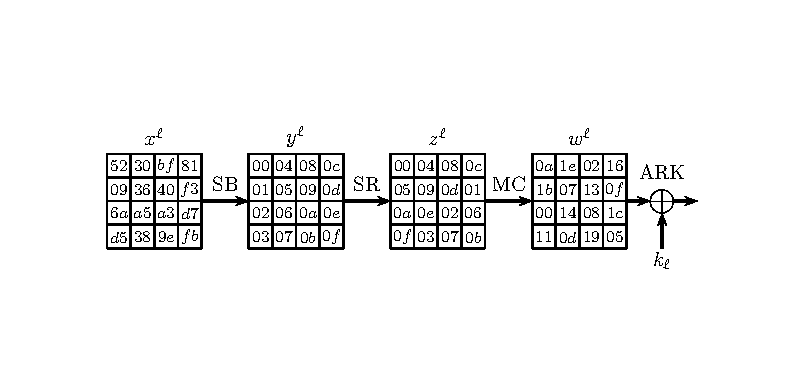
\includegraphics[trim = 10em 8em 10em 4em]{fig/AES-round.pdf}    
\end{center}
\caption{An AES Round}\label{fig:AESRound}
%\vspace*{-0.6cm}
\end{figure}

The rounds are numbered from $0$ to $Nr-1$, where $Nr$ is the number of rounds. The subkey used in the \ak operation of round~$\ell$ is denoted by $k^{\ell}$, and the $j$'th byte in its $i$'th row is denoted by $k^{\ell}_{4j+i}$. The whitening key added before the initial round is denoted by $k^{-1}$. The $j$'th byte in the $i$'th row of the state before the \subB, \sr, \mc, \ak operations of round~$\ell$ is denoted by $x^\ell_{4j+i}, y^\ell_{4j+i}, z^\ell_{4j+i},$ and $w^\ell_{4j+i}$, respectively.  A set of bytes $\left\{v_i, v_j, v_k\right\}$ is denoted by $v_{i,j,k}$.

\subsection{The Square Attack on AES}
\label{sec:sub:Square}

AES was designed as a modification of the block cipher Square~\cite{FSE:DaemenKR97}, which came together with a dedicated attack, called `the Square attack'. This attack, in its basic application to AES, uses the following observation.
\begin{lemma}\label{Lem:Square1}
Consider the encryption by 3-round AES of a set of 256 plaintexts, $P_0,P_1,\ldots,P_{255}$, which are equal in all bytes except for a single byte, such that the single byte assumes each possible value exactly once. Then the corresponding ciphertexts $C_0,C_1,\ldots,C_{255}$ satisfy $\bigoplus_{i=0}^{255} C_i=0$.  
\end{lemma}
As was shown in~\cite{FSE:DaemenKR97}, this property can be used to attack 6-round Square, and also 6-round AES, with a complexity of about $2^{80}$ S-box computations. The adversary asks for the encryption of $2^{32}$ plaintexts which are equal in all bytes except for the main diagonal (i.e., bytes 0,5,10,15) and assume all $2^{32}$ possible values in the main diagonal. Then, he guesses bytes $0,5,10,15$ of $k^{-1}$, and for each guess, he partially encrypts the plaintexts through round~0 and finds a set of $2^8$ inputs to round~1 which satisfy the assumption of Lemma~\ref{Lem:Square1}. Then, he partially guesses the subkeys $k^4,k^5$, partially decrypts the $2^8$ corresponding ciphertexts through rounds~4,5 and checks whether the XOR of the $2^8$ corresponding values at the state $x^4_0$ (i.e., at byte 0 before the \subB operation of round~4) is zero, as is stated by Lemma~\ref{Lem:Square1}. If not, the subkey guess is discarded.

While it seems that in order to compute byte $x^4_0$ from the ciphertext, the adversary must know 64 subkey bits (specifically, key bytes $k^5_{0,7,10,13}$ and $k^4_{0,1,2,3}$), in fact knowing 40 subkey bits is sufficient. Indeed, since \mc is a linear operation, it can be interchanged with the \ak operation after it, at the cost of replacing $k^4$ with the equivalent subkey $\bar{k}^4=\mc^{-1}(k^4)$. The knowledge of the key bytes $k^5_{0,7,10,13}$ and $\bar{k}^4_0$ is sufficient for computing the state byte $x^4_0$ from the ciphertext of 6-round AES.\footnote{Here and in the sequel, we assume that in 6-round AES, the \mc operation of round~5 is omitted. If this operation is not omitted, the attack works almost without change; we only have to replace the key $k^5$ with the equivalent key $\bar{k}^5=\mc^{-1}(k^5)$.} Each check whether $2^8$ values XOR to zero provides an 8-bit filtering, and hence, checking several sets is sufficient for discarding all wrong subkey guesses. The attack recovers 9 subkey bytes ($k^{-1}_{0,5,10,15},\bar{k}^4_0,k^5_{0,7,10,13}$) with complexity of about $2^{32} \cdot 2^{40} \cdot 2^8=2^{80}$ S-box computations.

In~\cite{FSE:FKLSSWW00}, Ferguson et al.~observed that the Square attack can be improved by replacing Lemma~\ref{Lem:Square1} with the following lemma on 4-round AES.
\begin{lemma}\label{Lem:Square2}
Consider the encryption by 4-round AES of a set of $2^{32}$ plaintexts, $P_0,P_1,\ldots,P_{2^{32}-1}$, which are equal in all bytes except for the main diagonal (i.e., bytes 0,5,10,15), such that the diagonal assumes each possible value exactly once. Then the corresponding ciphertexts $C_0,C_1,\ldots,C_{2^{32}-1}$ satisfy $\bigoplus_{i=0}^{2^{32}-1} C_i=0$.  
\end{lemma}
Lemma~\ref{Lem:Square2} can be used to attack 6-round AES using the same strategy described above. The adversary asks for the encryption of a few sets of $2^{32}$ plaintexts which satisfy the assumption of Lemma~\ref{Lem:Square2}. Then, for each set, he guesses subkey bytes $\bar{k}^4_0,k^5_{0,7,10,13}$ and checks whether the XOR of the $2^{32}$ intermediate values at the state byte $x^4_0$ is zero, as is stated by Lemma~\ref{Lem:Square2}. The attack recovers 5 subkey bytes ($\bar{k}^4_0,k^5_{0,7,10,13}$) and its complexity is about $2^{32} \cdot 2^{40}=2^{72}$ S-box computations.

\subsection{The Partial Sums Attack}
\label{sec:sub:partial-sums}

In the same paper~\cite{FSE:FKLSSWW00}, Ferguson et al.~showed that the complexity of the Square attack described above can be significantly reduced, by dividing the key guessing and partial decryption into several steps and gradually reducing the number of values whose XOR should be computed. By the structure of AES, the state byte $x^4_0$ is computed from the ciphertext $C$ using the following formula:
\begin{align}\label{Eq:Square1}
  \begin{split}
x^4_0=S^{-1}\big(\bar{k}^4_0 \oplus \hex{0e} \cdot &S^{-1}(C_0 \oplus k^5_0) \oplus \hex{09} \cdot S^{-1}(C_7 \oplus k^5_7) \oplus \\
&\oplus \hex{0d} \cdot S^{-1}(C_{10} \oplus k^5_{10}) \oplus \hex{0b} \cdot S^{-1}(C_{13} \oplus k^5_{13})\big),
  \end{split}  
\end{align}
where the coefficients $\hex{0e},\hex{09},\hex{0d},\hex{0b}$ come from the inverse \mc operation and the multiplication is performed in the finite field $GF(2^8)$. 

Note that the right hand side of~\eqref{Eq:Square1} depends only on bytes 0,7,10,13 of the ciphertext. This means that if two ciphertexts are equal in these four bytes, then their contributions to the XOR of $x^4_0$ values cancel each other. Thus, we may replace the list of ciphertexts with a list $A$ of $2^{32}$ binary indices which indicates whether each of the $2^{32}$ possible values of bytes 0,7,10,13 of the ciphertext appears an even or an odd number of times in the list of ciphertexts. The goal of the subsequent steps is to reduce the number of needed binary indices, in parallel to guessing subkey bytes. 

At the first step, the adversary guesses bytes 0,7 of $k^5$, and reduces the size of the list to $2^{24}$. Denote $a_1 = \hex{0e} \cdot S^{-1}(C_0 \oplus k^5_0) \oplus \hex{09} \cdot S^{-1}(C_7 \oplus k^5_7)$. Observe that if two ciphertexts are equal in the bytes $a_1,C_{10},C_{13}$, then their contributions to the XOR of $x^4_0$ values cancel each other. As the guess of bytes $k^5_{0,7}$ allows computing $a_1$ for each ciphertext, the adversary can construct a list $A_1$ of $2^{24}$ binary values which indicates whether each possible value of $(a_1,C_{10},C_{13})$ appears an even or an odd number of times in the list of intermediate values. The complexity of this step is about $2^{16} \cdot 2^{32}=2^{48}$ S-box evaluations.

At the second step, the adversary guesses the byte $k^5_{10}$ and reduces the list to a list $A_2$ of size $2^{16}$ that corresponds to the possible values of $(a_2,C_{13})$, where $a_2 = a_1 \oplus \hex{0d} \cdot S^{-1}(C_{10} \oplus k^5_{10})$. At the third step, the adversary guesses the byte $k^5_{13}$ and reduces the list to a list $A_3$ of size $2^{8}$ that corresponds to the possible values of $a_3$, where $a_3 = a_2 \oplus \hex{0b} \cdot S^{-1}(C_{13} \oplus k^5_{13})$. Finally, at the fourth step, the adversary guesses the byte $\bar{k}^4_0$, computes $\oplus_{\{x \in \{0,1\}^8:A_3[x]=1\}} S^{-1}(\bar{k}^4_0 \oplus x)$, which is equal to the right hand side of~\eqref{Eq:Square1}, and checks whether it is equal to zero. The complexity of each step is about $2^{48}$ S-box computations, and thus, the overall complexity for a single set of $2^{32}$ plaintexts is $2^{50}$ S-box computations. 

As the attack recovers 5 subkey bytes, six sets of $2^{32}$ plaintexts are required to recover their value uniquely with a high probability. Note that after the check of the first set, only about $2^{40} \cdot 2^{-8}=2^{32}$ suggestions for the 40 subkey bits remain undiscarded. This means that for each possible value of $k^5_{0,7,10,13}$, at most a few values of $\bar{k}^4_0$ that correspond to them are expected to remain. Hence, when examining the second set of $2^{32}$ plaintexts, the complexity of the fourth step becomes negligible as it is performed only for a few values of $\bar{k}^4_0$. Similarly, when examining the third set, the two last steps become negligible, etc. In total, the complexity of checking all six plaintext sets of size $2^{32}$ is equivalent to the cost of $4+3+2+1=10$ steps, or $2^{51.3}$ S-box computations.\footnote{We note that in~\cite{FSE:FKLSSWW00}, the authors performed a similar analysis and concluded that the complexity is $2^{52}$ S-box computations. This value was used in all subsequent papers. For the sake of consistency, we use the same value in Table~\ref{Tab:Results}, but note that the actual complexity is lower, as is shown here, and use the lower estimate when comparing the partial sums attack with our new attack.} 

The attack is given as Algorithm~\ref{alg:partial-sum}.
To simplify the notation, we rewrite equation~\eqref{Eq:Square1} in a more generic way, using
$S_0$ for $\hex{0e} \cdot S^{-1}(\cdot)$,
$S_1$ for $\hex{09} \cdot S^{-1}(\cdot)$,
$S_2$ for $\hex{0d} \cdot S^{-1}(\cdot)$,
$S_3$ for $\hex{0b} \cdot S^{-1}(\cdot)$,
and renaming the keys and the ciphertext bytes to $k_0, k_1, k_2, k_3, k_4$ and $c_0, c_1, c_2, c_3$, respectively:
\begin{equation}
    a_4 = S^{-1}\left(k_4 \oplus S_0(c_0 \oplus k_0) \oplus S_1(c_1 \oplus k_1) \oplus S_2(c_2 \oplus k_2) \oplus S_3(c_3 \oplus k_3)\right).
    \label{Eq:Square2}
\end{equation}

\begin{algorithm}[!ht]
    \begin{algorithmic}[1] % enter the algorithmic environment
        \State Input: Array $A$ of bits such that the $j^{\text{th}}$ value of $A$ denotes the parity of the number of occurrences of $j$ in the list of ciphertexts
            \ForAll{$k_0, k_1$}
            \State Declare an empty bit-array $A_1$ of size $2^{24}$
                \ForAll{$c_0, c_1, c_2, c_3$}
                    \If{$A[c_0, c_1, c_2, c_3] = 1$}
                        \State{$a_1 \gets S_0(c_0 \oplus k_0) \oplus S_1(c_1 \oplus k_1)$}
                        \State{$A_1[a_1, c_2, c_3] \gets A_1[a_1, c_2, c_3] \oplus 1$}
                    \EndIf
                \EndFor

                \ForAll{$k_2$}
                    \State Declare an empty bit-array $A_2$ of size $2^{16}$
                    \ForAll{$a_1, c_2, c_3$}
                        \If{$A_1[a_1, c_2, c_3] = 1$}
                            \State{$a_2 \gets a_1 \oplus S_2(c_2 \oplus k_2)$}
                            \State{$A_2[a_2, c_3] \gets A_2[a_2, c_3] \oplus 1$}
                        \EndIf
                    \EndFor

                    \ForAll{$k_3$}
                        \State Declare an empty bit-array $A_3$ of size $2^{8}$
                        \ForAll{$a_2, c_3$}
                            \If{$A_2[a_2, c_3] = 1$}
                                \State{$a_3 \gets a_2 \oplus S_3(c_3 \oplus k_3)$}
                                \State{$A_3[a_3] \gets A_3[a_3] \oplus 1$}
                            \EndIf
                        \EndFor

                        \ForAll{$k_4$}
                            \State {$a_4 \gets 0$}
                            \ForAll{$a_3$}
                                \If{$A_3[a_3] = 1$}
                                    \State $a_4 \gets a_4 \oplus S^{-1}(k_4 \oplus a_3)$
                                \EndIf
                            \EndFor
                            \If{$a_4 \ne 0$}
                                \State {$k_0, k_1, k_2, k_3, k_4$} is not a valid key candidate
                            \EndIf
                        \EndFor
                    \EndFor
             \EndFor
            \EndFor
    \end{algorithmic}
\caption{Partial-sum algorithm for key recovery~\cite{FSE:FKLSSWW00}.\label{alg:partial-sum}}
\end{algorithm}


\paragraph{Reducing the data complexity.} In~\cite{Tunstall12}, Tunstall observed that the data complexity of the attack can be reduced to $2^{33}$ chosen plaintexts by examining two sets of $2^{32}$ plaintexts instead of six sets. The idea is to check an analogue of Equation~\eqref{Eq:Square1} for three additional bytes -- $x^4_5, x^4_{10},$ and $x^4_{15}$ -- using the same set of $2^{32}$ plaintexts. Note that in order to compute each of these three bytes from the ciphertext, the adversary needs the subkey bytes $k^{5}_{0,7,10,13}$ (which are the same as in Equation~\eqref{Eq:Square1}), along with a different byte of $\bar{k}^4$. When two sets are checked at the same byte, they provide a 16-bit filtering, which in particular yields an 8-bit filtering on the value $k^{5}_{0,7,10,13}$ which is common to all examined bytes. Hence, information from different bytes can be combined to recover $k^5_{0,7,10,13}$ with a high probability. 

The data complexity can be further reduced to $2^{32}$ by examining a single set and checking the XOR in all 16 bytes of $x^4$. The algorithm is more complex and uses a meet-in-the-middle procedure based on the properties of the AES key schedule. We omit the description here, as it will not be needed in the sequel. 

In~\cite{Tunstall12}, it is claimed that when the same set of plaintexts is used to check the parity in several bytes, the complexity of checking the first byte is dominant, as some of the computations performed for computing the XOR in different bytes are identical. However, this claim seems incorrect, as in the variant of Equation~\eqref{Eq:Square1} for other bytes, the order of the coefficients 
$\hex{0e},\hex{09},\hex{0d},\hex{0b}$ which stems from the inverse \mc operation is changed, and hence, the operations performed for different bytes are not identical and only knowledge of subkeys can be `reused'. Therefore, the complexity of the attack that uses two sets is about $(4+3+2+2+1+1)\cdot 2^{48}=2^{51.7}$ S-box computations, and the attack that uses one set takes about $16 \cdot 2^{50}=2^{54}$ S-box computations.

The idea of using two sets of size $2^{32}$ instead of six was independently suggested in~\cite{alda2016implementation} by Alda et al., who also verified it experimentally.

%\subsection{Integral attacks against AES with partial sums}\label{sub:literature_partial_sum}

\iffalse
\NK{
Here is the list of the papers we directly compete with. Of course, we will have to explain exactly our gain over each of them.
\begin{itemize}
    \item[\cite{FSE:FKLSSWW00}] Ferguson, Kelsey, Lucks, Schneier, Stay, Wagner, and Whiting, Improved cryptanalysis of Rijndael, FSE 2000.
    \\The basic "partial sums" paper.\\
    \item[\cite{Tunstall12}] Tunstall, Improved “Partial Sums”-based Square Attack on AES, SeCrypt 2012, eprint:2012/280
    \\Claims that "partial sums" on 6-round AES can be improved by a factor of 2, by examining only two $\delta$-sets instead of 6 in the original paper. Also claims that a single $\delta$-set is sufficient, if the memory is increased to $2^{40}$. How does this compare to / combine with our results?\\
    \SG{Did not understand it completely, but if we can use it in our attack, we transform a $\times 6$ factor into a $\times 2$ in the overall complexity.}
    \item[\cite{EPRINT:AANS14}] Alda, Aragona, Nicolodi, and Sala, Implementation and Improvement of the Partial Sum Attack on 6-round AES, Physical and Data-Link Security Techniques for Future Communication Systems, 2016, eprint:2014/216
    \\Claims that "partial sums" on 6-round AES can be improved by a factor of 2, by examining only two $\delta$-sets instead of 6. The attack was practically verified. How does this compare to / combine with our results? 
\end{itemize}
}
\fi

\subsection{The FFT-Based Attack of Todo and Aoki}
\label{sec:sub:FFT-old}

The general idea of using the Fast Fourier Transform (FFT) for speeding up cryptanalytic attacks on block ciphers goes back to Collard et al.~\cite{ICISC:CollardSQ07} who used the FFT to speed up linear cryptanalysis. This idea was extended to several other techniques, including multi-dimensional linear attacks~\cite{ACISP:NguyenWWL10,ACISP:NguyenWW11}, zero-correlation attacks~\cite{SAC:BGWWC13}, differential-linear attacks~\cite{C:BeierleLT20}, etc.
%
In~\cite{CANS:TodAok14}, Todo and Aoki proposed to replace the partial sums technique by an FFT-based technique. The basic idea behind the Todo-Aoki technique is that the sum of the values in the right hand side of Equation~\eqref{Eq:Square1} which we want to compute can be written in the form of a \emph{convolution} of tailor-made functions, as seen in Algorithm~\ref{alg:fht-todo}. 

Consider a set $S$ of $2^{32}$ ciphertexts for which we want to compute the XOR of the intermediate values at the state byte $x^4_0$. Like in the partial sums attack, denote by $A$ a bit array of size $2^{32}$, such that $A(c_0,c_1,c_2,c_3)=1$ if and only if $C_{0,7,10,13}=(c_0,c_1,c_2,c_3)$ holds for an odd number of ciphertexts in $S$. Let $f:\{0,1\}^{32} \to \{0,1\}$ be the indicator function of the array, that is, $f(c_0,c_1,c_2,c_3)=\indic(A(c_0,c_1,c_2,c_3)=1)$. Assume that the subkey $k_4$ was guessed, and let $g_i:\{0,1\}^{32} \to \{0,1\}$, for $0\leq i \leq 7$, be defined by 
%\begin{align}\label{Eq:Fourier1}
%  \begin{split}
%g_i(t_0,t_1,t_2,t_3)=[S^{-1}(\bar{k}^4_0 \oplus \hex{0e} \cdot &S^{-1}(t_0) \oplus \hex{09} \cdot S^{-1}(t_1) \oplus \\
%&\oplus \hex{0d} \cdot S^{-1}(t_2) \oplus \hex{0b} \cdot S^{-1}(t_3))]_i,
%  \end{split}  
%\end{align}
\begin{equation}\label{Eq:Fourier1}
g_i(t_0,t_1,t_2,t_3)=\left[S^{-1}\left(k_4 \oplus S_0(t_0) \oplus S_1(t_1) \oplus
S_2(t_2) \oplus S_3(t_3)\right)\right]_i,
\end{equation}
where $[S^{-1}(t)]_i$ denotes the $i$'th bit of $S^{-1}(t)$. Then, denoting by $[x(C,k_0,k_1,k_2,k_3)]_i$ the $i$'th bit of the value $x^4_0$ corresponding to the ciphertext $C$ for a given guess of $k_0,k_1,k_2,k_3$ (see Equation~\eqref{Eq:Square2}), we have
%\begin{align}
%    \begin{split}
%    \bigoplus_{C \in S} &[x^4_0(C)]_i = \bigoplus_{\{(c_0,c_1,c_2,c_3):A[c_0,c_1,c_2,c_3]=1\}} g_i(c_0 \oplus k_0,c_1 \oplus k_1,c_2 \oplus k_3, c_3 \oplus k_4) \\
%    &= \bigoplus_{(c_0,c_1,c_2,c_3) \in \{0,1\}^{32}} f(c_0,c_1,c_2,c_3) g_i(c_0 \oplus k^5_0,c_1 \oplus k^5_7,c_2 \oplus k^5_{10}, c_3 \oplus k^5_{13}) \\
%    &= (f * g_i)(k^5_0,k^5_7,k^5_{10},k^5_{13}).
%    \end{split}
%\end{align}
\begin{align}
\begin{split}
    \bigoplus_{C \in S} \left[x(C,k_0,k_1,k_2,k_3)\right]_i
    &= \bigoplus_{\mathmakebox[6em][c]{\{(c_0,c_1,c_2,c_3):A[c_0,c_1,c_2,c_3]=1\}}} g_i(c_0 \oplus k_0,c_1 \oplus k_1,c_2 \oplus k_2, c_3 \oplus k_3) \notag \\
    &= \bigoplus_{\mathclap{c_0,c_1,c_2,c_3}} f(c_0,c_1,c_2,c_3) \cdot g_i(c_0 \oplus k_0,c_1 \oplus k_1,c_2 \oplus k_2, c_3 \oplus k_3) \\
    &= (f * g_i)(k_0,k_1,k_2,k_3).
\end{split}
\end{align}
Therefore, we can compute the sum for all $2^{32}$ possible guesses of $(k_0,k_1,k_2,k_3)$ at once by guessing the byte $k_4$ and computing the convolution of two functions on 32 bits, that takes time of about $4 \cdot 2^{32} \log_2(2^{32})$ additions, as was shown by Collard et al.~\cite{ICISC:CollardSQ07}. As the summation is performed for each bit separately, the complexity of examining a single set $S$ of $2^{32}$ ciphertexts is $8 \cdot 2^8 \cdot 4 \cdot 2^{32} \log_2(2^{32}) = 2^{50}$ additions, which is roughly equal to the number of operations required for examining a single set of ciphertexts in the partial sums attack.

A disadvantage of the Todo-Aoki technique, compared to the partial sums attack, is that it cannot use partial knowledge of the subkey to obtain a speedup. Indeed, as the computation is performed for all values of $(k_0,k_1,k_2,k_3)$ at the same time, partial knowledge (e.g., knowledge of $k_3$) cannot be exploited. As a result, when six sets of $2^{32}$ ciphertexts are examined, the complexity of the Todo-Aoki attack becomes $6 \cdot 2^{50}=2^{52.6}$ additions, while the overall complexity of partial sums is only $2^{51.3}$ S-box computations, as was shown above.

The question, whether there is a way to use partial knowledge of the key in an FFT-based attack, was explicitly mentioned as an open question in~\cite{CANS:TodAok14}.

\begin{algorithm}[tb!]
    \begin{algorithmic}[1] % enter the algorithmic environment
        \State Input: Array $A$ of bits such that the $j^{\text{th}}$ value of $A$ denotes the parity of the number of occurrences of $j$ in the list of ciphertexts
            \ForAll{$k_4$}
            \tcb{
                \ForAll{$k_0, k_1, k_2, k_3$}
                    \State 
                         {$\displaystyle A_1[k_1, k_2, k_3, k_4] \gets
                        \bigoplus\limits_{\mathclap{c_0, c_1, c_2, c_3}} A[c_0, c_1, c_2, c_3]\cdot
                        S^{-1}\left(\begin{gathered}k_4 \oplus S_0(c_0 \oplus k_0) \oplus S_1(c_1 \oplus k_1)\\ \oplus S_2(c_2 \oplus k_2) \oplus S_3(c_3 \oplus k_3)\end{gathered}\right)\hspace*{-2cm}$}
                \EndFor
                }
                \ForAll{$k_0, k_1, k_2, k_3$}
                     \If{$A_1[k_0, k_1, k_2, k_3] \neq 0$}
                         \State {$k_0, k_1, k_2, k_3, k_4$} is not a valid key candidate
                     \EndIf
                \EndFor
            \EndFor
    \end{algorithmic}
\caption{FFT-based algorithm for key recovery~\cite{CANS:TodAok14}.\\
The \tcb{blue} colored step has naive complexity $2^{32}\times2^{32}$, but can be replaced by several Hadamard transformations of size $2^{32}$ with complexity $2^{37}$ each.\label{alg:fht-todo}}
\end{algorithm}


\paragraph{Using precomputation of the FFT to speed up the attack.} In the eprint version of the same paper~\cite{EPRINT:Todo14}, Todo showed that the complexity of the attack can be reduced by precomputing some of the Fast Fourier Transforms that should be computed in the course of the attack.

Recall that the computation of the convolution of $f,g:\{0,1\}^n \to \{0,1\}$ using the FFT consists of three stages:
\begin{enumerate}[leftmargin=0.1in]
    \item Computing the Fourier transforms $\hat{f},\hat{g}: \{0,1\}^n \to \mathbb{Z}$.
    \item Computing the pointwise product $h:\{0,1\}^n \to \mathbb{Z}$ defined by $h(x)=\hat{f}(x) \cdot \hat{g}(x)$.
    \item Computing the inverse Fourier transform (which is the same as computing the Fourier transform and dividing by $2^n$) to obtain $f * g = \hat{h} \cdot 2^{-n}$.
\end{enumerate}
Here, we use the convention that the Fourier transform $\hat{f}$ is obtained from $f$ by writing $f$ as a $2^n$-dimensional vector and multiplying it by the Hadamard matrix $H_n$, defined recursively as $H_n=\big(\begin{smallmatrix}
  H_{n-1} & H_{n-1} \\
  H_{n-1} & -H_{n-1}
\end{smallmatrix}\big)$, where 
$H_1=\big(\begin{smallmatrix}
  1 & 1\\
  1 & -1
\end{smallmatrix}\big)$. 

The cost of each computation of the FFT is $n2^n$ addition operations.  In order to avoid overflow the additions should have at least $2n$ bits of precision, but since we only want one bit of the result the computation can be done with $n+1$ bits of precision.  For the 6-round AES attack we have $n=32$ and the FFT will typically be implemented with 64-bit additions.  The cost of the pointwise product is about $2^n$ multiplication operations, which is not much more than the cost of $2^n$ addition operations for small $n$ (in particular for a software implementation with $n \leq 32$, as in the attack on 6-round AES).\footnote{We note that in~\cite{CANS:TodAok14}, the authors conservatively estimate that pointwise multiplication of two vectors of size $2^n$ whose entries are $n$-bit integers takes $n2^n$ addition operations. For the sake of consistency with~\cite{CANS:TodAok14} and fairness, we use the conservative estimate in the table of results and the less conservative estimate when we compare the Todo-Aoki technique to our technique.} Hence, the overall cost of the convolution computation in our case is about $3 \cdot 32 \cdot 2^{32}$ additions.   

\enlargethispage{\baselineskip}

Todo observed that the Fourier transforms $\hat{f}$ and $\hat{g}$ can be precomputed. As the function $f$ does not depend on the guess of $k_4$, one can compute it once, store the result (which requires at most $2^{32}$ 64-bit words), and re-use it for each value of $k_4$. As the cost of this FFT computation is $32 \cdot 2^{32}$ additions, the amortization over guesses of $k_4$ makes it negligible. The function $g$ cannot be precomputed since it depends on $k_4$. On the other hand, as it does not depend on the ciphertexts, it can be reused for other sets of ciphertexts. Therefore, the complexity of computing the XOR for a single set of $2^{32}$ ciphertexts is reduced to about $8 \cdot 2^8 \cdot 2 \cdot 32 \cdot 2^{32} = 2^{49}$ addition operations, and the complexity of computing the XOR for six sets is reduced to about $2^{49}+5 \cdot 2^{48} = 2^{50.8}$ addition operations. If only two sets are examined and the XOR is computed in four bytes (as was described above), then the complexity becomes $2^{49}+7 \cdot 2^{48} = 2^{51.2}$ addition operations. This complexity seems a bit lower than the complexity of partial sums, but it is still quite close and the different types of operations make comparison between the techniques tricky.

\iffalse
\NK{
\begin{itemize}
    \item[\cite{CANS:TodAok14}] Todo and Aoki, FFT Key Recovery for Integral Attack, CANS 2014
    \\The paper we compete with. Contains also background on previous FFT-based techniques which we will have to cite. Contains the idea of precomputing values that will be used more than once, but works with 6 delta-sets. Asks as an open problem whether there is way to exploit key dependence in FFT-based partial sums. Our technique solves this.
\end{itemize}
}


\begin{table}[!ht]
    \centering
    \begin{tabular}{|c|c|c|c|c|}
        \hline
        ~\AES-version-\#rounds~ & ~time~ & ~\# $\Delta$-set~ & ~memory~ & ~source~ \\ \hline\hline
        \rule{0pt}{2ex}\multirow{7}{*}{\AES-128-6r}  & $2^{}$ &  & $2^{}$ & original \\ \cline{2-5}
        \rule{0pt}{3ex} & $2^{51.7}$ & 6 & $2^{41.58}$ & \cite{CANS:TodAok14} \iffalse this is the paper of Todo on the FFT \fi \\ \cline{2-5}
        \rule{0pt}{3ex} & $2^{50.7}$ & & $2^{}$ & \cite{ACISP:Tunstall09} \\\cline{2-5}
        \rule{0pt}{3ex} & $2^{50.17}$ & 6 & ~$2^{42.58}$ & Sec.~\ref{} \\\cline{2-5}
        \rule{0pt}{3ex} & $2^{49.59}$ & 6 & $2^{41}$ & Sec.~\ref{} \\\cline{2-5}
        \multirow{3}{*}{\AES-192} & & & & \\ \hline
        &&&& \\ \cline{2-5}
        &&&& \\ \hline
        \multirow{3}{*}{\AES-256]} &&&& \\ \cline{2-5}
        &&&& \\ \cline{2-5}
        &&&& \\\hline
    \end{tabular}
    \vspace*{0.2cm} % to separate the table from the caption
    \caption{Sum-up of the complexity of the partial-sum like attacks against \AES in the literature.}
    \label{tab:complexity_comparaison}
\end{table}
\fi


\section{The New Technique: Partial Sums Meet FFT}\label{sec:new_attack}

In this section, we describe our new technique which allows combining the advantages of the partial sums technique with those of the Todo-Aoki FFT-based technique. We begin with a basic variant of the technique in Section~\ref{sec:sub:basic}, then we show how the complexity can be reduced significantly by packing several FFT computations together in Section~\ref{sec:sub:packing}, afterward, we present several additional enhancements and other variants of the basic technique in Section~\ref{sec:sub:improvements}, and we conclude this section with a comparison of our technique with partial sums and the Todo-Aoki technique in Section~\ref{sec:sub:comparison}. For the sake of concreteness, we present the attack in the case of 6-round AES and reuse the notations of Section~\ref{sec:background}. It will be apparent from the description how our technique can be applied in general.

\subsection{The Basic Technique}\label{sec:sub:basic}

Our basic observation is that we can follow the general structure of the partial sums attack, and replace each step by computing a convolution of properly chosen functions. This is shown in Algorithm~\ref{alg:fht-basic} which is a rearrangement of the operations of Algorithm~\ref{alg:partial-sum}, making convolution appear. As we use somewhat different convolutions for different steps of the attack, we present them separately.  

\subsubsection{First step.} As described in Section~\ref{sec:sub:partial-sums}, before the first step of the partial sums attack, the list of ciphertexts is replaced with a list $A$ of $2^{32}$ binary indices which indicate whether each of the $2^{32}$ possible values of the bytes $c_0,c_1,c_2,c_3$ appears an even or an odd number of times in the list of ciphertexts. At the first step, the adversary guesses the bytes $k_0,k_1$, and replaces the list by a list $A_1$ of size $2^{24}$ which corresponds to the bytes $a_1,c_2,c_3$, where $a_1 = S_0(c_0 \oplus k_0) \oplus S_1(c_1 \oplus k_1)$. 

We observe that the list $A_1$ can be computed for all values $k_0,k_1$ simultaneously by computing a convolution. Let $\chi:\{0,1\}^{32} \to \{0,1\}$ be the indicator function of the list $A$. That is, $\chi(c_0,c_1,c_2,c_3)=1$ if and only if the value $(C_0,C_7,C_{10},C_{13})=(c_0,c_1,c_2,c_3)$ appears an odd number of times in the list of ciphertexts. For any $c_2,c_3 \in \{0,1\}^8$, define
$
\chi^1_{c_2,c_3}(c_0,c_1)=\chi(c_0,c_1,c_2,c_3).
$

\noindent For any $a_1 \in \{0,1\}^8$, let $I^1_{a_1}(x,y)=\indic(S_0(x) \oplus S_1(y) = a_1).$
Both $\chi^1_{c_2,c_3}$ and $I^1_{a_1}$ are indicator functions on $\{0,1\}^{16}$. For any $a_1,c_2,c_3 \in \{0,1\}^8$, we have
\begin{align*}
    (\chi^1_{c_2,c_3} * I^1_{a_1})(k_0,k_1) &= \sum_{\mathclap{c_0,c_1 \in \{0,1\}^8}} \chi^1_{c_2,c_3}(c_0,c_1) \cdot I^1_{a_1}(c_0 \oplus k_0,c_1 \oplus k_1) \\
    &= \sum_{\mathclap{c_0,c_1 \in \{0,1\}^8}} \chi(c_0,c_1,c_2,c_3) \cdot \indic(S_0(c_0 \oplus k_0) \oplus S_1(c_1 \oplus k_1) = a_1).
\end{align*}
Therefore, the entry which corresponds to $(a_1,c_2,c_3)$ in the list $A_1[k_0, k_1]$ created for the subkey guess $(k_0,k_1)$ is 
\begin{align}
    A_1[k_0, k_1][a_1,c_2,c_3]=\left((\chi^1_{c_2,c_3} * I^1_{a_1})(k_0,k_1)\right) \bmod 2.
\end{align}
(Note that formally, we define $A_1$, which is a list of size $2^{24}$ that depends on two key bytes, as an array of size $2^{16} \times 2^{24}$ which includes the guessed bytes.) As was shown in Section~\ref{sec:sub:FFT-old}, the computation of this convolution requires $3 \cdot 16 \cdot 2^{16}$ addition operations for each value of $a_1,c_2,c_3$, or a total of $48 \cdot 2^{40}$ additions. This compares favorably with the first step of the partial sums attack which requires $2^{48}$ S-box computations. As we shall see below, the actual advantage of our technique is significantly larger. However, this requires to store the full $A_1$ for all values of $(k_0,k_1)$, of size $2^{40}$ bits.

\subsubsection{Second step.} At the second step of the partial sums attack, the adversary guesses the byte $k_2$ and reduces the list $A_1$ to a list $A_2$ of size $2^{16}$ that corresponds to the possible values of $(a_2,c_3)$, where $a_2 = a_1 \oplus S_2(c_2 \oplus k_2)$. 

We compute the entries of the list $A_2$ using a convolution, as follows. For any $k_0,k_1,c_3 \in \{0,1\}^8$, define
\begin{align*}
\chi^2_{k_0,k_1,c_3}(a_1,c_2) &= \indic(A_1[k_0, k_1][a_1,c_2,c_3]) &
I^2(x,y) &= \indic(x=S_2(y)).
\end{align*}
Both $\chi^2_{k_0,k_1,c_3}$ and $I^2$ are indicator functions on $\{0,1\}^{16}$. For any $k_0,k_1,c_3 \in \{0,1\}^8$, we have
\begin{align*}
    (\chi^2_{k_0,k_1,c_3} * I^2)(a_2,k_2) &= \sum_{\mathclap{a_1,c_2 \in \{0,1\}^8}} \chi^2_{k_0,k_1,c_3}(a_1,c_2) \cdot I^2(a_1 \oplus a_2,c_2 \oplus k_2) \\
    &= \sum_{\mathclap{a_1,c_2 \in \{0,1\}^8}} \indic(A_1[k_0, k_1][a_1,c_2,c_3]) \cdot \indic(a_1 \oplus a_2 = S_2(c_2 \oplus k_2))\\
    &= \sum_{\mathclap{a_1,c_2 \in \{0,1\}^8}} \indic(A_1[k_0, k_1][a_1,c_2,c_3]) \cdot \indic(a_2 = a_1 \oplus S_2(c_2 \oplus k_2)).
\end{align*}
Therefore, the entry which corresponds to $(a_2,c_3)$ in the list $A_2$ created for the subkey guess $(k_0,k_1,k_2)$ is 
\begin{align}
    A_2[k_2][a_2,c_3]=\left((\chi^2_{k_0,k_1,c_3} * I^2)(a_2,k_2)\right) \bmod 2.
\end{align}
(Note that formally, we define $A_2$, which is a list of size $2^{16}$ that depends on three key bytes, as an array of size $2^{8} \times 2^{16}$, which depends on $k_0,k_1$). As above, the complexity of this step is $48 \cdot 2^{40}$ additions.

\subsubsection{Third step.} This step is similar to the second step. Thus, we present it briefly.
At the third step of the partial sums attack, the adversary guesses the byte $k_3$ and reduces the list $A_2$ to a list $A_3$ of size $2^{8}$ that corresponds to the possible values of $a_3$, where $a_3 = a_2 \oplus S_3(c_3 \oplus k_3)$. We obtain the list $A_3$ by defining
$$
\chi^3_{k_0,k_1,k_2}(a_2,c_3) = \indic(A_2[k_2][a_2,c_3]) \qquad \mbox{and} \qquad I^3(x,y) = \indic(x=S_3(y)),
$$
and setting
\begin{align}
    A_3[k_3][a_3]=\left((\chi^3_{k_0,k_1,k_2} * I^3)(a_3,k_3)\right) \bmod 2.
\end{align}
(Note that formally, we define $A_3$ as an array of size $2^{8} \times 2^8$, which depends on $k_0,k_1,k_2$). As above, the complexity of this step is $48 \cdot 2^{40}$ additions.

\subsubsection{Fourth step.} At the fourth step of the partial sums attack, the adversary guesses the byte $k_4$, and computes $\oplus_{\{x \in \{0,1\}^8:A_3[x]=1\}} S^{-1}(k_4 \oplus x)$, which is equal to the right hand side of~\eqref{Eq:Square2}, and checks whether it is equal to zero. 

We cannot compute this XOR directly using a convolution, since in order to apply the FFT we need functions whose output is an integer and not an element of $GF(2^8)$. A basic solution, that was adopted by Todo and Aoki~\cite{CANS:TodAok14}, is to compute the XOR in each bit separately. To this end, we define the functions $\chi^4_{k_0,k_1,k_2,k_3},I^{4,j}:\{0,1\}^8 \to \{0,1\}$ for $j=0,1,\ldots,7$ by
$$
\chi^4_{k_0,k_1,k_2,k_3}(a_3) =1(A_3[k_3][a_3]) \qquad \mbox{and} \qquad I^{4,j}(x)=[S^{-1}(x)]_j,
$$
where $[S^{-1}(x)]_j$ denotes the $j$'th bit of $S^{-1}(x)$. We have
\begin{align*}
        (\chi^4_{k_0,k_1,k_2,k_3} * I^{4,j})(k_4) &= \sum_{\mathclap{a_3 \in \{0,1\}^8}} \chi^4_{k_0,k_1,k_2,k_3}(a_3) \cdot I^{4,j}(a_3 \oplus k_4) \\
        &= \sum_{\mathclap{a_3 \in \{0,1\}^8}} \indic(A_3[k_3][a_3]) \cdot [S^{-1}(a_3 \oplus k_4)]_j.
\end{align*}
Therefore, the $j$'th bit of the XOR we would like to compute for the key guess $(k_0,k_1,k_2,k_3,k_4)$ is equal to 
\begin{equation}\label{Eq:New1}
\left((\chi^4_{k_0,k_1,k_2,k_3} * I^{4,j})(k_4)\right)\bmod 2.
\end{equation}
Hence, we can check the XOR by initializing a list of $2^{40}$ binary indicators which correspond to the possible values of $(k_0,k_1,k_2,k_3,k_4)$, computing the convolutions $\chi^4_{k_0,k_1,k_2,k_3} * I^{4,j}$ for $j=0,1,\ldots,7$, and discarding all keys $(k_0,k_1,k_2,k_3,k_4)$ for which at least one of the results of~\eqref{Eq:New1} is not equal to zero modulo 2.

The complexity of this step is $2^{32} \cdot 8 \cdot (3 \cdot 8 \cdot 2^8) = 192 \cdot 2^{40}$ additions, which is slightly better than the complexity of the fourth step of the partial sums technique. As we shall show below, the complexity can be reduced significantly, by using a new method to pack several FFT together, and exploiting enhancements from previous attacks based on the re-use of computations.

\begin{algorithm}[t]
    \begin{algorithmic}[1] % enter the algorithmic environment
        \State Input: Array $A$ of bits such that the $j^\text{th}$ value of $A$ denotes the parity of ciphertext $j$
        
        \State Declare an empty 2D bit-array $A_1$ of size $2^{16} \times 2^{24}$; \Comment{$2^{40}$ memory}
         
            \ForAll{$a_1, c_2, c_3$}
            \tcb{
                \ForAll{$k_0$, $k_1$}
                    \State 
                         {$\displaystyle A_1[k_0, k_1][a_1, c_2, c_3] \gets 
                        \bigoplus\limits_{\mathclap{c_0, c_1}} A[c_0, c_1, c_2, c_3]\cdot \indic(S_0(c_0 \oplus k_0) \oplus S_1(c_1 \oplus k_1) = a_1)$}
                \EndFor
                    }
            \EndFor
        \ForAll{$k_0, k_1$}
            \State Declare an empty 2D bit-array $A_2$ of size $2^{8}\times2^{16}$;
                \ForAll{$c_3$}
                \tcb{
                    \ForAll{$k_2, a_2$}
                    \State 
                    {$\displaystyle A_2[k_2][a_2,c_3] \gets 
                        \bigoplus\limits_{\mathclap{a_1, c_2}} A_1[k_0, k_1][a_1, c_2, c_3]\cdot \indic(a_1 \oplus S_2(c_2 \oplus k_2) = a_2)$}
                    \EndFor
                }
                \EndFor
            \ForAll{$k_2$}
                \State Declare an empty 2D bit-array $A_3$ of size $2^{8}\times 2^{8}$;
                    \color{blue}
                    \ForAll{$k_3, a_3$}
                    \State 
                    { $\displaystyle A_3[k_3][a_3] \gets 
                        \bigoplus\limits_{\mathclap{a_2, c_3}} A_2[k_2][a_2,c_3]\cdot \indic(a_2 \oplus S_3(c_3 \oplus k_3) = a_3)$}
                    \EndFor
                    \color{black}
                    \ForAll{$k_3$}
                    \State Declare an empty 1D byte-array $A_4$ of size $2^{8}$;
                        \color{red}
                        \ForAll{$k_4$}
                            \State {
                            $\displaystyle A_4[k_4] \gets 
                                \bigoplus\limits_{a_3} A_3[k_3][a_3]\cdot S^{-1}(a_3\oplus k_4)$}
                        \EndFor
                        \color{black}
                       \ForAll{$k_4$}
                            \If{$A_4[k_4] \neq 0$}
                                \State {$k_0, k_1, k_2, k_3, k_4$} is not a valid key candidate
                            \EndIf
                       \EndFor
                \EndFor
            \EndFor
        \EndFor
    \end{algorithmic}
\caption{The following is the Algorithm for key recovery. The function $\indic$ is the indicator function. All the \tcb{blue} colored steps are of complexity $2^{16}\times2^{16}$ and can be replaced by a $3$ Hadamard transformations of size $2^{16}$ with total complexity $3 \times 2^{20}$. The \tcr{red} colored step has complexity $2^8 \times 2^8$, which can be replaced by $3$ Hadamard transformations of size $2^{8}$ with total complexity $3 \times 2^{11}$.\label{alg:fht-basic}}
\end{algorithm}


\subsection{Packing Several FFTs Together by Embedding into $\mathbb{Z}$}
\label{sec:sub:packing}

We now show that the complexity of the basic attack can be significantly reduced by packing several convolution computations into a single convolution.  We assume that the attack is implemented using 64-bit operations, which is typical for a software implementation.  For reference, the 6-round AES attack of Todo and Aoki requires 64-bit additions to avoid overflow.

\subsubsection{Improving the fourth step of the attack.} Consider the fourth step of our basic attack described above. The step consists of computing the convolution of the function $\chi^4_{k_0,k_1,k_2,k_3}$ with the eight functions $I^{4,j}$ ($j=0,1,\ldots,7$). These eight convolutions can be replaced by a single computation of convolution. 

Let $s$ be a `separation parameter' that will be determined below, and define a function $I^4:\{0,1\}^8 \to \mathbb{Z}$ by
$
I^4(x) = \sum_{j=0}^7 2^{js} [S^{-1}(x)]_j.
$

We claim that for an appropriate choice of $s$, the convolution $\chi^4_{k_0,k_1,k_2,k_3} * I^{4}$ allows recovering the value of the XOR in all 8 bits we are interested in, with a high probability. Indeed, we have

\begin{align*}
      (\chi^4_{k_0,k_1,k_2,k_3} * I^{4})(k_4) &= \sum_{\mathclap{a_3 \in \{0,1\}^8}} \chi^4_{k_0,k_1,k_2,k_3}(a_3) \cdot I^{4}(a_3 \oplus k_4) \\
      &=  \sum_{\mathclap{a_3 \in \{0,1\}^8}} \indic(A_3[k_3][a_3]) \cdot \sum_{j=0}^7 2^{sj} [S^{-1}(a_3 \oplus k_4)]_j \\
      &=\sum_{j=0}^7 2^{sj} \sum_{a_3 \in \{0,1\}^8} \indic(A_3[k_3][a_3]) \cdot [S^{-1}(a_3 \oplus k_4)]_j \\ 
      &=  \sum_{j=0}^7 2^{sj} (\chi^4_{k_0,k_1,k_2,k_3} * I^{4,j})(k_4), 
\end{align*}
where the penultimate equality uses the change of the order of summation. 

Recall that for each value of $k_4$, we want to compute the eight parity bits 
$(\chi^4_{k_0,k_1,k_2,k_3} * I^{4,j}(k_4))\bmod 2$. Let us reformulate our goal, for the sake of convenience. Denoting $b_j=\chi^4_{k_0,k_1,k_2,k_3} * I^{4,j}(k_4)$, we have $\chi^4_{k_0,k_1,k_2,k_3} * I^{4}(k_4)=\sum_{j=0}^7 2^{sj}b_j$. Thus, for non-negative integers $b_0,b_1,\ldots,b_7$, we are given $\sum_{j=0}^7 2^{sj}b_j$ and we want to compute from it the eight parity bits $(b_j)\bmod 2$. 

Observe that if for all $0 \leq j \leq 7$, we have $b_j<2^s$, then the multiplications by $2^{sj}$ separate the values $b_j$, and thus, we can simply read the values $(b_j)\bmod 2$ from $2^{sj}b_j$, as in this case,
$$
\forall j: \left[\sum_{j=0}^7 2^{sj}b_j\right]_{sj} = [2^{sj}b_j]_{sj} = (b_j)\bmod 2.
$$
\paragraph{How large should $s$ be so that $b_j<2^s$ holds with a high probability for all $j$'s?} Note that each $b_j$ is the sum of 128 elements, which correspond to the 128 values of $c_3$ such that $[S^{-1}(c_3 \oplus k_4)]_j=1$. Each such element is $\chi^4_{k_0,k_1,k_2,k_3}(c_3)$, which can be viewed as a randomly distributed indicator. Hence, $b_j$ is distributed like $Bin(128,1/2)$. The expectation of such a variable is 64, and its standard deviation is $4\sqrt{2}$. This means that the values $b_j$ are strongly concentrated around 64, and the probability $\Pr[b_j\geq 2^7]$ is extremely small. Therefore, by taking $s=7$, we can derive the eight parity bits $(b_j)\bmod 2$ from the sum $\sum_{j=0}^7 2^{sj}b_j$, easily and with a very low error probability.
\paragraph{How small should $s$ be in order to perform the entire computation with 64-bit words?} For the sake of efficiency, we compute the convolution using 64-bit word operations and disregard overflow beyond the $64$'th bit. If $s$ is too large, this may cause an error in the computation of the sum $\sum_{j=0}^7 2^{sj}b_j$, and consequently, in the computation of the parity bits $(b_j)\bmod 2$. 

To overcome this, note that in the computation of a convolution of $f,g:\{0,1\}^n \to \mathbb{Z}$, all operations are additions and multiplications, except for division by $2^n$ at the last step. Hence, when we neglect overflow beyond the $64$'th bit, this causes an additive error of $m \cdot 2^{64}$ for some $m \in \mathbb{Z}$ until the last step, and an additive error of $m \cdot 2^{64-n}$ at the final result. Assuming that $b_j<2^{s}$ for all $j$, this error does not affect the parity bits as long as $7s<64-n$ (as the error affects only the top $n$ bits of $\sum_{j=0}^7 2^{sj}b_j$). 

In our case, $n=8$ and hence, for all $s \leq 7$, the possible error does not affect the parity bits we compute.

\paragraph{Reducing $s$ even further.} Note that we can allow random errors in the convolution computations that do not correspond to the right subkey guess, as such random errors do not increase the probability of a wrong key guess to pass the filtering. Hence, we only have to make sure that for the right key, we obtain the correct value of the parity bits with a high probability.

As was explained above, the values $b_j$ are concentrated around 64.
Formally, by evaluating the cumulative distribution function of the binomial law, we have $\Pr[48 < b_j < 80] >0.99$, and thus, $0<b_j-48<2^5$ with a very high probability.
To make use of this concentration, we subtract from the value  $\sum_{j=0}^7 2^{sj}b_j$ the integer $u=48\sum_{j=0}^7 2^{sj}$, to obtain 
$$
\sum_{j=0}^7 2^{sj}b_j - \sum_{j=0}^7 48 \cdot 2^{sj} = \sum_{j=0}^7 (b_j-48)2^{sj}. 
$$
Since $0<b_j-48<2^5$, we can compute the parity bits $(b_j)\bmod 2$ also for $s=6$ and for $s=5$, with a very low error probability.
\paragraph{Summary of improving the fourth step.} To summarize, the eight convolutions can be computed using a single convolution of functions over $\{0,1\}^8$. This reduces the complexity of this step to $2^{32} \cdot 3 \cdot 8 \cdot 2^8 = 24 \cdot 2^{40}$ operations.

\subsubsection{Improving the other steps of the attack.} Once we acquired the ability to compute several convolutions in parallel, we can use it at the other steps of the attack as well. The idea is to pack the convolutions that correspond to several subkey guesses into a single convolution. We exemplify this approach by showing how the first step of the attack can be improved; the improvement of the second and the third steps is similar. 

Recall that at the first step of our attack, for any values $c_2,c_3 \in \{0,1\}^8$, we compute the parity of the convolution
$(\chi^1_{c_2,c_3} * I^1_{a_1})(k_0,k_1)$, for all $k_0,k_1 \in \{0,1\}^8$. We may pack up to seven such computations in parallel. For example, in order to pack four computations, we write $c_2=(c_2^h,c_2^l)$, where $c_2^h$ denotes the two most significant bits of $c_{2}$ and is identified with an integer between 0 and 3, via the binary expansion. We define
$$
\chi^1_{c_2^h,c_2^l,c_3}(c_0,c_1)=\chi(c_0,c_1,c_2,c_3), \text{ and } \bar{\chi}^{1}_{c_2^l,c_3}=\sum_{j=0}^3 2^{sj} \chi^1_{j,c_2^l,c_3}.
$$

Then, for any $c_2^l \in \{0,1\}^6$, and $k_0,k_1,c_3 \in \{0,1\}^8$, we compute the convolution
$(\bar{\chi}^1_{c_2^l,c_3} * I^1_{a_1})(k_0,k_1)$, and using the technique described above we derive from it the four parity bits $((\chi^1_{c_2,c_3} * I^1_{a_1})(k_0,k_1)) \bmod 2$ with $c_2 \in \{(0, c_2^l), \ldots, (3,c_2^l)\}$.

To see what is the maximal value of $s$ we may take, note that each convolution value $b'=(\chi^1_{c_2,c_3} * I^1_{a_1})(k_0,k_1)$ is the sum of 256 elements, which correspond to the 256 values of $(c_0,c_1)$ such that $S_0(c_0 \oplus k_0) \oplus S_1(c_1\oplus k_1)=a_1$. Each such element can be viewed as a randomly distributed indicator. Hence, $b'$ is distributed like $Bin(256,1/2)$.  When analyzing step 4, we could tolerate a low probability of errors for the right key, but in the first step, there are $2^{24}$ values of $A_1$ that are involved in the computation for the right key, and we want all of them to be correct.  Therefore, we use $s \ge 7$, since $\Pr[64<b'<192]>1-2^{-50}$.
Hence, by subtracting $64 \cdot \sum_{j=0}^3 2^{js}$ from the convolution value $(\bar{\chi}^1_{c_2^l,c_3} * I^1_{a_1})(k_0,k_1)$, we can compute the parity bits $\left((\chi^1_{c_2,c_3} * I^1_{a_1})(k_0,k_1)\right) \bmod 2$ with a very high probability for $s \geq 7$, and the $2^{24}$ relevant values are simultaneously correct with probability at least $1-2^{-26}$.

Unfortunately, with $s = 7$ we can only pack 7 parallel convolutions within 64-bit words.  Indeed, at this step, the convolution is computed for functions over $\{0,1\}^{16}$ (instead of 8-bit functions in the fourth step), and thus, we would need $7s<64-16=48$ in order to pack 8 FFTs and avoid errors due to overflow. 
(We exemplified the idea of packing 4 parallel convolutions for the sake of convenience).

This reduces the complexity of the first step of the attack from $2^{24} \cdot 3 \cdot 16 \cdot 2^{16} = 48 \cdot 2^{40}$ to $48/7 \cdot 2^{40}$ addition operations. The complexity of the second step can be reduced similarly from $48 \cdot 2^{40}$ to $48/7 \cdot 2^{40}$.  For the third step, we can actually use $s=6$ and pack 8 parallel convolutions within a 64-bit word, because we only need $2^8$ correct computations, and we have $\Pr[96<b'<160]^{256}>0.98$; the complexity is reduced from $48 \cdot 2^{40}$ to $6 \cdot 2^{40}$.

\subsubsection{Improving the fourth step even further.} Finally, we can reduce the complexity of the fourth step even further by packing 12 FFTs in a 64-bit word with $s=5$. This requires to change the way we do the packing: instead of packing 8 different $I^{4,j}$ with a fixed $\chi^4$ as was described above, we consider each function $I^{4,j}$ separately and pack a fixed $I^{4,j}$ with 12 $\chi^4$ functions corresponding to different key guesses. This reduces the complexity of the fourth step from $24 \cdot 2^{40}$ to $16 \cdot 2^{40}$.

\subsection{Enhancements and Other Variants of the Basic Technique}
\label{sec:sub:improvements}

In this section, we present two enhancements that reduce the complexity of the attack, along with another variant of the technique that provides us with flexibility that will be useful in the application of our technique to other ciphers.

\subsubsection{Precomputing some of the FFT computations.} At each step of the attack, we perform three FFT computations. As was described in Section~\ref{sec:sub:FFT-old} regarding the FFT-based attack of Todo and Aoki, some of these computations do not depend on the guessed key material, and hence, they can be precomputed at the beginning of the attack, thus reducing the overall time complexity. 

Specifically, the functions $I^2,I^3,I^4,$ and $I^1_{a_1}$ (for all $a_1 \in \{0,1\}^8)$ do not depend on any guessed subkey bits, and thus, their FFTs can be precomputed with overall complexity of about $2^8 \cdot 16 \cdot 2^{16}=2^{28}$ addition operations, which is negligible compared to other steps of the attack. The results can be stored in lists that require about $2^{24}$ 64-bit words of memory.

The function $\chi^1_{c_2,c_3}$ does not depend on the value of $a_1$, and thus, its FFT can be computed once (for each value of $(c_2,c_3)$) and reused for all values of $a_1$. This reduces the time complexity of this FFT computation (in total, for all values of $c_2,c_3$) to $2^{16} \cdot 16 \cdot 2^{16}=2^{36}$ additions, which is negligible compared to other steps of the attack. As we need to store in memory at each time only the result of the FFT that corresponds to a single value of $c_2,c_3$, the memory requirement of this step is $2^{16}$ 64-bit words of memory. 

These precomputations reduce the time complexity of the first step (in which two FFTs can be precomputed) from $48/7 \cdot 2^{40}$ to $16/7 \cdot 2^{40}$ additions, the time complexity of the second, third, and fourth steps (in which one FFT can be precomputed) to $32/7 \cdot 2^{40}, 4 \cdot 2^{40},$ and $32/3 \cdot 2^{40}$ additions, respectively. 

If the fourth step is implemented by packing 12 $\chi^4$ functions together, as was described above, we can reduce its complexity further by precomputing the FFT of the function $\bar{\chi}^4$ which represents the `packed' function and reusing it for computing convolutions with the eight functions $I^{4,j}$ ($j=0,1,\ldots,7$). This reduces the time complexity of the fouth step to $(16+(16/8))/3 \cdot 2^{40} = 6 \cdot 2^{40}$ additions.

Therefore, the time complexity of examining a set of $2^{32}$ plaintexts is reduced to $2^{40} \cdot (16/7+32/7+4+6) \approx 16.9 \cdot 2^{40} \approx 2^{44.1}$ additions. 

\subsubsection{Lower cost for examining additional sets of plaintexts.} As was described in Section~\ref{sec:sub:partial-sums} regarding the partial sums attack, when we check the XOR of additional sets of $2^{32}$ values at a byte which we already checked for one set, the complexity of the check is reduced. Indeed, after the first set was checked, we expect that for each value of $(k^5_0,k^5_7,k^5_{10},k^5_{13})$, only a few values of $\bar{k}^4_0$ are not discarded. Hence, instead of performing the fourth step of the attack by computing a convolution, we can simply compute the sum directly for each of the remaining candidate subkeys. The average complexity of such a step is $2^{32} \cdot 1 \cdot 2^{7}=2^{39}$ S-box evaluations and the same number of XORs, which is equivalent to about $1 \cdot 2^{40}$ addition operations. Note that since the fourth step is the most time consuming step of our attack, this gain is more significant than the gain which the partial sums attack achieves in the same case.

After two sets were checked, we expect that for each value of $(k^5_0,k^5_7,k^5_{10})$, only a few values of $(k^5_{13},\bar{k}^4_0)$ are not discarded. Hence, instead of performing the third and the fourth steps of the attack by computing convolutions, we can simply directly perform each of them for each of the remaining candidate subkeys. This reduces the complexity of the third step to $2^{40}$ additions and the complexity of the fourth step to $2^{32}$ additions.

\paragraph{Attack that examines six sets of $2^{32}$ plaitexts.} By continuing the reasoning in the same manner, we see that the complexity of considering six sets of $2^{32}$ ciphertexts and computing the XOR of the values $x^4_0$ that correspond to them, is about
\[
\begin{gathered}
2^{40}\cdot\left(\left(\frac{16+32}{7}+4+6\right)+\left(\frac{16+32}{7}+4+1\right)+\left(\frac{16+32}{7}+1\right)+\left(\frac{16}{7}+1\right)+1\right) \\ \approx 40.8 \cdot 2^{40} \approx 2^{45.4} \text{ additions.} 
\end{gathered}
\]


\paragraph{Attack that examines two sets of $2^{32}$ plaitexts.} If we consider two sets of $2^{32}$ ciphertexts and examine 4 different bytes (as was suggested by Tunstall~\cite{Tunstall12} for the partial sums attack), then we may begin with checking the XOR of both sets at the byte $x^4_{0}$, which requires $2^{40}(16.9+11.9)$ additions as was described above. Then, we must move to another byte, and it seems that we have to pay a `full price' again. However, note that after the first two filterings, for each value of $(k^5_0,k^5_7,k^5_{10})$ we are left with one value of $k^5_{13}$ on average. As these four subkey bytes are reused in the examination of the XOR in the byte $x^4_5$ (along with a different byte from $\bar{k}^4$), we can replace the third step by computing the sum directly for each remaining value of $k^5_{13}$ and replace the fourth step by computing the sum directly for each remaining value of $(k^5_{13},\bar{k}^4_1)$. This reduces the complexity of each of these two steps to $2^{40}$ additions. When we examine the second set of $2^{32}$ ciphertexts at the byte $x^4_5$, the complexity of the fourth step can be further reduced to $2^{32}$ additions, since for any value of $(k^5_0,k^5_7,k^5_{10})$ we are left with one value of $(k^5_{13},\bar{k}^4_1)$ on average.   

Continuing in the same manner, we see that the complexity of considering two sets of $2^{32}$ ciphertexts and computing the XOR of the values $x^4_{0,5,10,15}$ that correspond to them, is about
\[
\begin{gathered}
2^{40}\cdot\Big(\left(\frac{16+32}{7}+4+6\right)+\left(\frac{16+32}{7}+4+1\right)+
\left(\frac{16+32}{7}+1+1\right)+\\ \left(\frac{16+32}{7}+1\right)+
\left(\frac{16}{7}+1\right)+\left(\frac{16}{7}+1\right)+
1\Big) \approx 62.8 \cdot 2^{40} \approx 2^{46} \text{ additions.}
\end{gathered}
\]


\paragraph{Attack that examines one set of $2^{32}$ plaintexts.} As was explained in Section~\ref{sec:sub:partial-sums}, in this case we examine each byte with only a single set of ciphertexts, and thus, we do not obtain information that can be reused in other computations. Therefore, the complexity of our attack in this case is $16 \cdot 16.9 \cdot 2^{40} = 2^{48.1}$ addition operations, which is 16 times the complexity of checking a single set of ciphertexts (like in the partial sums and the Todo-Aoki attacks with only a single set of $2^{32}$ ciphertexts examined). 

\subsubsection{Alternative Way of Performing the First Step.} Recall that at the first step we are given a list $A$ of $2^{32}$ binary indices which correspond to $(c_0,c_1,c_2,c_3)$ and our goal is to compute the $2^{24}$ entries of the list $A_1$ which corresponds to triples of the form $(a_1,c_2,c_3)$ where $a_1 = S_0(c_0 \oplus k_0) \oplus S_1(c_1 \oplus k_1)$, for all values of $(k_0,k_1)$. We may divide this step into two sub-steps as follows:
\begin{itemize}
    \item \emph{Step~1.1:} At this sub-step, we guess the subkey $k_0$ and update the list $A$ into a list $A_0$ of $2^{32}$ binary indices that correspond to $(a_0,c_1,c_2,c_3)$, where $a_0=S_0(c_0 \oplus k_0)$. The complexity of this step is about $2^{32} \cdot 2^8 =2^{40}$ S-box computations.

    \item \emph{Step~1.2:} At this sub-step, performed for each guess of $k_0$, our goal is to replace the list $A_0$ with a list of size $2^{24}$ that corresponds to the values $(a_1,c_2,c_3)$ where $a_1 = a_0 \oplus S_1(c_1 \oplus k_1)$, for each value of $k_1$. This task is exactly the same as the task handled at the second and third steps of our attack described above, and hence, it can be performed in exactly the same way. Specifically, the convolution we have to compute is 
    \begin{gather}
    A_1[k_0, k_1][a_1,c_2,c_3]=\left((\bar{\chi}^1_{k_0,c_2,c_3} * \bar{I}^1)(a_1,k_1)\right) \bmod 2,
    \shortintertext{where}
    \bar{\chi}^1_{k_0,c_2,c_3}(a_0,c_1) = \indic(A_0(a_0,c_1,c_2,c_3)=1), \mbox{   and   } \bar{I}^1(x,y) = \indic(x=S_1(y)). \notag
\end{gather}
    Like in the second step of our attack described above, we can precompute one FFT and perform the computation of 7 FFTs in parallel. Hence, the complexity of this sub-step is $32/7 \cdot 2^{40}$ additions. 
    \end{itemize}
The alternative version of the attack is present in Algorithm~\ref{alg:fht-lowmem}.

\begin{algorithm}[t]
    \begin{algorithmic}[1] % enter the algorithmic environment
        \State Input: Array $A$ of bits such that the $j^\text{th}$ value of $A$ denotes the parity of ciphertext $j$
        
        \ForAll{$k_0$}
            
            \State Declare an empty 1D bit-array $A_0$ of size $2^{32}$; \Comment{$2^{32}$ memory}
                \ForAll{$c_0, c_1, c_2, c_3$}
                    \State $a_0 \gets S_0(c_0 \oplus k_0)$
                    \State $A_0[a_0, c_1, c_2, c_3] \gets A[c_0, c_1, c_2, c_3]$
                \EndFor
            \State Declare an empty 2D bit-array $A_1$ of size $2^{8} \times 2^{24}$; \Comment{$2^{32}$ memory}
            \ForAll{$c_2, c_3$}
            \tcb{
                \ForAll{$k_1, a_1$}
                    \State 
                         {$\displaystyle A_1[k_1][a_1, c_2, c_3] \gets 
                        \bigoplus\limits_{\mathclap{a_0, c_1}} A_0[a_0, c_1, c_2, c_3]\cdot \indic(a_0 \oplus S_1(c_1 \oplus k_1) = a_1)$}
                \EndFor
                    }
            \EndFor
        \ForAll{$k_1$}
            \State Declare an empty 2D bit-array $A_2$ of size $2^{8}\times2^{16}$;
                \ForAll{$c_3$}
                \tcb{
                    \ForAll{$k_2, a_2$}
                    \State 
                    {$\displaystyle A_2[k_2][a_2,c_3] \gets 
                        \bigoplus\limits_{\mathclap{a_1, c_2}} A_1[k_1][a_1, c_2, c_3]\cdot \indic(a_1 \oplus S_2(c_2 \oplus k_2) = a_2)$}
                    \EndFor
                }
                \EndFor
            \ForAll{$k_2$}
                \State Declare an empty 2D bit-array $A_3$ of size $2^{8}\times 2^{8}$;
                    \color{blue}
                    \ForAll{$k_3, a_3$}
                    \State 
                    { $\displaystyle A_3[k_3][a_3] \gets 
                        \bigoplus\limits_{\mathclap{a_2, c_3}} A_2[k_2][a_2,c_3]\cdot \indic(a_2 \oplus S_3(c_3 \oplus k_3) = a_3)$}
                    \EndFor
                    \color{black}
                    \ForAll{$k_3$}
                    \State Declare an empty 1D byte-array $A_4$ of size $2^{8}$;
                        \color{red}
                        \ForAll{$k_4$}
                            \State {
                            $\displaystyle A_4[k_4] \gets 
                                \bigoplus\limits_{a_3} A_3[k_3][a_3]\cdot S^{-1}(a_3\oplus k_4)$}
                        \EndFor
                        \color{black}
                       \ForAll{$k_4$}
                            \If{$A_4[k_4] \neq 0$}
                                \State {$k_0, k_1, k_2, k_3, k_4$} is not a valid key candidate
                            \EndIf
                       \EndFor
                \EndFor
            \EndFor
        \EndFor
    \EndFor
    \end{algorithmic}
\caption{Low-memory version of the attack.\label{alg:fht-lowmem}}
\end{algorithm}


Formally, the complexity of the alternative way is higher than the complexity of the original way of performing this step described above --- $39/7 \cdot 2^{40}$ additions instead of $16/7 \cdot 2^{40}$ additions. As a result, the complexity of the attack with two sets of $2^{32}$ plaintexts becomes about $82.5 \cdot 2^{40} \approx 2^{46.4}$ additions (which is the complexity we mention in the introduction). However, this alternative has several advantages:
\begin{enumerate}
    \item \emph{Lower memory complexity.} In the attack described above, the most memory-consuming part is the first step which requires a list of $2^{40}$ bit entries. Thus, its memory complexity is about $2^{33}$ 128-bit blocks. 

    The alternative way reduces the memory complexity of the first step to $2^{32}$ bits. We observe that all other steps of the attack can be performed with at most $2^{34}$ bits of memory. Indeed, all ciphertexts can be transformed immediately into entries of the table $A$ whose size is $2^{32}$ bits. The table $A_0$ (which should be stored for one value of $k_0$ at a time) requires $2^{32}$ bits. The subsequent tables used in the attack are smaller, and the arrays used in the FFTs are also smaller (as all FFTs are performed on 16-bit or 8-bit functions). By checking two sets of $2^{32}$ plaintexts in parallel, we reduce the number of remaining keys after examining the byte $x^4_0$ to $2^{24}$, and then the storage of these keys requires less than $2^{30}$ bits of memory. Therefore, the total memory complexity of the attack is reduced to about $2 \cdot 2^{32} + 2^{32}<2^{34}$ bits, i.e., $2^{27}$ 128-bit blocks.

    \item \emph{Lower average-case time complexity.} While it is common to measure the complexity of attacks using the worst-case scenario (e.g., the complexity of exhaustive search over an $n$-bit key is computed as $2^n$, although on average, the attack finds the key after $2^{n-1}$ trials), the average-case complexity has clear practical significance. In the partial sums attack and in the Todo-Aoki attack, the average-case time complexity is half of the worst-case complexity, since the attack is applied for $2^8$ `external' guesses of a subkey, and the right key is expected to be found after trying half of these subkeys. In the original version of our attack, since the last step is performed for all keys in parallel, our average-case complexity is no better than the worst-case complexity, and so, we lose a factor of 2. In the alternative way described here, the attack is performed for each guess of the subkey $k^5_0$, and hence, we regain the factor 2 loss in the average-case complexity.

    \item \emph{Practical effect on the time complexity.} The lower memory complexity of the alternative variant of the attack is expected to have an effect on the time complexity as well. Indeed, our experiments show that the memory accesses to the $2^{40}$-bit sized array slow down our attack considerably. As the alternative variant requires only $2^{34}$ bits of memory, it may be even faster in practice than the original variant. 
 \end{enumerate}
The alternative way of performing the first step is also used in our improved attack on the full MISTY1~\cite{MISTY1} presented in the full version of this paper \cite{fullversion} in Appendix~A.

\subsection{Our Technique vs. Partial Sums and the Todo-Aoki Technique}\label{sec:sub:comparison}

In this section, we present a comparison between our new technique and the partial sums technique and the Todo-Aoki FFT-based technique. First, we discuss the case of 6-round AES, and then we discuss applications to general ciphers.

\subsubsection{The case of 6-round AES.} Here, we considered three attacks:
\begin{enumerate}
    \item \emph{Attack with 6 structures of $2^{32}$ chosen plaintexs.} The partial sums attack requires $2^{51.3}$ S-box computations, the Todo-Aoki attack requires $2^{50.8}$ additions, and our attack requires $2^{45.4}$ additions. Hence, our attack is at least 32 times faster than both previous attacks. In the experiments presented in Section~\ref{sec:sub:experiment}, the advantage of our attack was even bigger.

    \item \emph{Attack with 2 structures of $2^{32}$ chosen plaintexs.} The partial sums attack requires $2^{51.7}$ computations, the Todo-Aoki attack requires $2^{51.2}$ additions, and our attack requires $2^{46}$ additions. Hence, our attack is at least 32 times faster than both previous attacks.

    \item \emph{Attack with 1 structure of $2^{32}$ chosen plaintexs.} The partial sums attack requires $2^{54}$ S-box computations, the Todo-Aoki attack requires $2^{53}$ additions, and our attack requires $2^{48.1}$ additions. Hence, our attack is almost 32 times faster than both previous attacks. 
\end{enumerate}

\subsubsection{General comparison.} The speedup of our technique over the partial sums technique stems from two advantages: First, we replace key guessing steps with computation of convolutions. Second, we may pack the computation of several convolutions in a single convolution computation. The effect of the first advantage depends on the number of subkey bits guessed at the most time consuming steps of the attack: For a 4-bit subkey guess our gain is negligible, for an 8-bit key guess we get a speedup by a factor of more than 10 (without using packing), and for a 32-bit key guess our speedup factor may be larger than $2^{25}$ as is demonstrated in our attack on CLEFIA~\cite{CLEFIA} presented in Appendix~B of the full version of this paper~\cite{fullversion}. The effect of the second advantage is also dependent on the number of guessed subkey bits (since it determines the size of the functions whose convolution we have to compute, which in turn affects the number of convolutions we may pack together). Usually, between 4 and 8 convolutions can be packed together, which leads to a speedup by a factor of at least 4. Interestingly, when the number of guessed subkey bits is small (e.g., 4 bits), more convolutions can be packed together, and hence, a stronger effect of the second advantage compensates for a weaker effect of the first advantage. 

The speedup of our technique over the Todo-Aoki technique stems from two advantages: First, our attack provides us with more flexibility, meaning that instead of replacing the whole attack by a single FFT-based step, we can consider each step (or group of steps) of the partial sums procedure separately and decide whether it will be better to perform it with key guessing or with an FFT-based technique. Second, we may pack the computation of several convolutions in a single convolution computation. The first advantage allows us to make use of partial knowledge of the subkey. A particular setting in which this advantage plays a role is analysis of additional plaintext sets after one set was used to obtain some key filtering. While our technique and the partial sums technique can make use of this partial knowledge, the Todo-Aoki technique must repeat the entire procedure. In the case of 6-round AES, this makes our attack 6 times faster than the Todo-Aoki attack without using packing. A more complete comparison between our method and the Todo-Aoki technique is available in Appendix~D if the full version of this paper~\cite{fullversion}. 

The second advantage provides a speedup by a factor of at least 4, as was described above. Yet another advantage that is worth mentioning is that while the Todo-Aoki technique applies the FFT to functions in high dimensions (e.g., dimension 72 in the Todo-Aoki attack on 12-round CLEFIA-128 presented in~\cite{CANS:TodAok14}), our technique applies the FFT to functions of a significantly lower dimension (e.g., dimension 16 in our improved attack on 12-round CLEFIA-128 presented in Appendix~B of the full version of this paper~\cite{fullversion}). Computation of the FFT in high dimensions is quite cumbersome from the practical point of view, and hence, avoiding this is a practical advantage of our technique.  Moreover, higher dimension FFTs require additions with more precision; without using packing the Todo-Aoki attack on 6-round AES requires 64-bit additions while our attack can use 32-bit additions.

Two advantages of the partial sums technique and the Todo-Aoki technique over our technique are a somewhat lower memory complexity (about $2^{27}$ 128-bit blocks for partial sums and about $2^{31}$ 128-bit blocks for Todo-Aoki) and the fact that on average, the attack finds the right key after trying half of the possible keys while our attack must try all keys. However, both advantages can be countered by implementing the first step of our attack in the alternative way presented in Section~\ref{sec:sub:improvements}, which makes the memory complexity equal to that of the partial sums attack and regains the `lower average-case complexity', as was explained in Section~\ref{sec:sub:improvements}.

\subsection{Experimental Verification of Our Attack on 6-round AES} 
\label{sec:sub:experiment}

We have experimentally verified our attack on Amazon's AWS infrastructure. For comparison, we also implemented the partial sums attack of~\cite{FSE:FKLSSWW00} and the Todo-Aoki attack~\cite{CANS:TodAok14}. 
All implementations in C are publicly available at the following link: 
\[
    \text{\href{https://github.com/ShibamCrS/Partial\_Sums\_Meet\_FFT}{https://github.com/ShibamCrS/Partial\_Sums\_Meet\_FFT}.}
\]
We note that the FFT implementations were based on the ``Fast Fast Hadamard Transform'' library~\cite{FFHT-Library}. 

\subsubsection{The AWS instances used in the experiment.} For each attack we had to pick the most optimal AWS instance, depending on the computational and memory requirements. 

The partial sums attack is quite easy to parallelize, and its memory requirement is low. (Specifically, the memory requirement is $2^{34}$ bits, or 16GB, as was shown above. Furthermore, only an $2^{32}$-bit list that stores the parities of $(c_0,c_1,c_2,c_3)$ combinations should be stored in a memory readable by all threads). As a result, we took the Intel-based instance (that has the AES-NI instruction set) with the maximal number of cores per US\$. At the time the experiment was performed (January, 2023) this was the m6i.32xlarge instance.\footnote{The m6i.32xlarge instance has 128 Intel-based vCPUs and 512GB of RAM.}

For our attack (in its original variant) and for the Todo-Aoki attack, we needed instances that support a large amount of memory. The optimal choice for our attack was the same instance as the one for the partial sums attack --- the m6i.32xlarge instance. For the Todo-Aoki attack, we needed 64 GB of RAM for each thread of the attack. Hence, the optimal instance we found was the r6i.32xlarge instance.\footnote{The r6i.32xlarge instance has 128 Intel-based vCPUs and 1024GB of RAM.} We note that in the Todo-Aoki attack, we do not exploit all the vCPUs, but we do exploit the whole memory space (of 1 TB of RAM).

\subsubsection{Experimental results.} The partial sums attack took \timePartial minutes to complete, and its cost was \pricePartial US\$ (we used the US-east-2 region (Ohio) which offered the cheapest cost-per-hour for a Linux machine of~6.144 US\$, before VAT). The Todo-Aoki approach took \timeFFT minutes to complete, and its cost was~\priceFFT US\$ (at 8.064 US\$ per hour).
We note that due to the costs of these attacks, they were run only once, but none of those attacks (nor our attack) is expected to show high variance in the running time.

To evaluate the running time of our attack, we ran Algorithm~\ref{alg:fht-basic} and Algorithm~\ref{alg:fht-lowmem} ten times each. In both algorithms, we used only 4 FFTs packed in parallel at each of Steps~1,2,3 and 8 FFTs packed in parallel at Step~4, for ease of implementation. The average running time of Algorithm~\ref{alg:fht-basic} is 90 minutes, and its average cost is 9.21 US\$. The average running time of Algorithm~\ref{alg:fht-lowmem} is \timeOur minutes and its cost is \priceOur US\$. Hence, in the experiment our attack was \cheapup-times cheaper and \speedup times faster than both partial sums and Todo-Aoki's attacks. 




%\section{Implementation of the new partial-sum attack on 6 rounds \AES}\label{sec:attack_aes}
%\begin{algorithm}[t]
    \begin{algorithmic}[1] % enter the algorithmic environment
        \State Input: Array $\mathcal{X}$ of bits such that the $j-th$ value of $\mathcal{X}$ denotes the parity of ciphertexts $j$
        
        \State Declare an empty 2D bit-array $A[][]$ of size $2^{24}\times2^{16}$; \Comment{$2^{40}$ memory}
         
            \For{$c_3c_2a=0;c_3c_2a<2^{24};c_3c_2a=c_3c_2a+1$}
            \tcb{
                \For{ $k_1k_0=0;k_1k_0<2^{16};k_1k_0=k_1k_0+1$ }
                    \State 
                         {\tiny  $ \displaystyle A[c_3c_2a][k_1k_0] = 
                        \sum_{ c_1c_0 \in \{0,2^{16}-1\} } \mathcal{X}_i[c_3c_2c_1c_0]\cdot \mathcal{I}(a = S_0(c_0 \oplus k_0) \oplus S_1(c_1 \oplus k_1) )$}
                \EndFor
                    }
            \EndFor
        \For{$k_1k_0 = 0; k_1k_0 < 2^{16}; k_1k_0 = k_1k_0 + 1$}
            \State Declare an empty 2D bit-array $B[][]$ of size $2^{8}\times2^{16}$;
                \For{$c_3=0;c_3<2^{8};c_3=c_3+1$}
                \tcb{
                    \For{ $k_2b=0;k_2b<2^{16};k_2b=k_2b+1$ }
                    \State 
                    {\tiny $B^{\prime}[i][c_3][k_2b] = 
                        \sum_{ c_2a \in \{0,2^{16}-1\} } \mathcal{A}[i][k_1k_0][c_3c_2a]\cdot \mathcal{I}(a \oplus b = S_2(c_2 \oplus k_2))$}
                    \EndFor
                }
                \EndFor
            \For{$k_2 = 0; k_2 < 2^{8}; k_2 = k_2 + 1$}
                \State Declare an empty 1D bit-array $\mathcal{C}[]$ of size $2^{16}$;
                    \tcb{
                    \For{ $k_3c=0;k_3c<2^{16};k_3c=k_3c+1$ }
                    \State 
                    { $\mathcal{C}[i][k_3c] = 
                        \sum_{ c_3b \in \{0,2^{16}-1\} } \mathcal{B}[i][k_2][c_3b]\cdot \mathcal{I}(c \oplus b = S_3(c_3 \oplus k_3))$}
                    \EndFor
                    }
                    \For{$k_3 = 0; k_3 < 2^{8}; k_3 = k_3 + 1$}
                    \State Declare an empty 1D bit-array $\mathcal{S}[]$ of size $2^{8}$;
                        \For{$i=0;i<d;i=i+1$} 
                        \tcr{
                            \For{ $k_4=0;k_4<2^{8};k_4=k_4+1$ }
                            \State 
                            $\mathcal{S}[k_4] = 
                                \sum_{ c \in \{0,2^{8}-1\} } \mathcal{C}[k_3][c]\cdot S^{-1}(c\oplus k_4))$
                            \EndFor
                        }
                       \EndFor
                       \For{$k_4 = 0; k_4 < 2^{8}; k_4 = k_4 + 1$}
                            \If{$\mathcal{S}[k_4] \neq 0$}
                                \State $RK[k_4k_3k_2k_1k_0] = 1$
                            \EndIf
                       \EndFor
                \EndFor
            \EndFor
        \EndFor
    \end{algorithmic}
\caption{The following is the Algorithm for key recovery. The function $\mathcal{I}$ is the indicator function. All the \tcb{blue} colored steps are of complexity $2^{16}\times2^{16}$ and can be replaced by a $3$ Hadamard transformations of size $2^{16}$ with total complexity $3 \times 2^{20}$. The \tcr{red} colored step has complexity $2^8 \times 2^8$, which can be replaced by $3$ Hadamard transformations of size $2^{8}$ with total complexity $3 \times 2^{11}$. Note that we need XOR of $8$ bit values from the last Hadamard transformation. Here I have used Gaetan's trick with \tcr{$7$} bit separation that needs exactly $64$ bits. \label{alg:fht}}
\end{algorithm} 

%\subsection{Explantion of Gaetan's trick}
%Here let us explain the last \tcr{red} color $\mathsf{for}$ loop in the Algorithm~\ref{alg:fht}. We are basically computing a convolution of two function $f:\mathbb{F}_2^8 \to \mathbb{F}_2$ and $g:\mathbb{F}_2^8 \to \mathbb{F}_2^8$ such that
%\begin{align*}
%    f(c) = \begin{cases}
%       1, \text{ if $\mathcal{C}[i][k_3][c] = 1$ for some fixed $i$ and $k_3$}\\
%       0, \text{ otherwise} 
%    \end{cases}
%\end{align*} 
%and
%\begin{align*}
%    g(x) = S^{-1}(x).
%\end{align*} 

%So the convolution we are interested in is $f*g(k) = \sum_{c \in \mathbb{F}_2^8} f(c)g(c \oplus k)$ (However, in the end we need sum over $\mathbb{F}_2^8$, not over $\mathbb{Z}$, will deal with it later). We need to compute the above convolution for all $k \in \mathbb{F}_2^8$.

%Computing the convolution for all $k$ is actually a matrix-vector multiplication. The vector is $V = (f(0),....,f(2^8-1))$ and the matrix is $M$ where $M(i,j) = g(i\oplus j)$. Beacuse of the \emph{blockwise circular} property of the matrix we have the following equation
%\[
%M\cdot V = (1/2^8)H(H(C_1)\times H(V)) 
%\]
%where $H$ is a $2^8 \times 2^8$ Hadamard matrix and $C_1$ is the first column of $M$. These are the three Hadamard transformations that we need to compute.

%As the Hadamard matrix is over $\mathbb{Z}$ and not over $\mathbb{F}_2^8$, we can not compute the XOR sum as desired. So Todo's idea is to consider $g(x) = (g_0(x),...,g_7(x))$ and compute eight matrix-vector multiplications separately and finally combine them. Here Gaetan suggested considering a single matrix; however, each bit of each matrix element is separated by a few bits. For example if $M_{0x5,0x6} = g(0x5\oplus 0x6) = 0xFF$ and we consider $7$ bits seperation, then we write this as
%{\small$$00000000-0000001-0000001-0000001-0000001-0000001-0000001-0000001-0000001$$}

%\subsection{Experiment Detail}
%I tested the idea with random vectors $V$. I compute the following two things:
%\begin{itemize}
%   \item $U_1 = MV$, i.e., the convolution directly
%   \item $U_2 = (1/2^8)H(H(C_1)\times H(V))$ with $6,7$ or $8$ bit seperation
%\end{itemize}
%With a $7$ bit separation, I am always getting $U_1 = U_2$. However, for $6$ and $8$ bit separation I am always getting some positions of $U_1$ and $U_3$ are not equal.
%\subsection{Description of the attack}\label{sub:description_new_attack}

%The new attack with 6 $\Delta$-sets

%\subsection{Complexity analysis}\label{sub:complexity_new_attack}


%\subsection{Reducing the number of $\Delta$-sets}\label{sub:complexity_new_attack}



%\subsection{Experimental verification}\label{sub:experimental_verification}



\section{Improved Attack on Kuznyechik}\label{sec:other_target}

The flexibility of our techniques improves attacks against various other ciphers that use the partial sums technique. In this section, we demonstrate this by presenting an attack on 7-round Kuznyechik, which improves over the multiset-algebraic attack on the cipher presented in~\cite{TOSC:BirKhoPer16} by a factor of more than 80.  In the supplementary material of the full paper \cite{fullversion}, we present improved attacks on the full MISTY1 (App.~A), and variants of CLEFIA-128 with 11 and 12 rounds (App.~B). Our attacks on Kuznyechik and MISTY1 are the best known attacks on these ciphers. 

\subsection{The structure of Kuznyechik} 

The block cipher Kuznyechik~\cite{Kuznyechik} is the current encryption standard of the Russian Federation.  It is an SPN operating on a 128-bit state organized as a $4\times4$ array of 8-bit words. The key length is 256 bits, and the encryption process is composed of 9 rounds. Each round of Kuznyechik is composed of three operations: \begin{itemize} 
    \item[] \textbf{Substitution}. Apply an 8-bit S-box independently to every byte of the state; 
    \item[] \textbf{Linear Transformation}. Multiply the state by an invertible 16-by-16 matrix $M$ over $GF(2^8)$;
    \item[] \textbf{Key Addition}. XOR a 128-bit round key computed from the secret key to the state.
\end{itemize}
An additional key addition operation is applied before the first round. As properties of the key schedule of Kuznyechik are not used in this paper, we omit its description and refer the reader to~\cite{Kuznyechik}.

\subsection{The multiset-algebraic attack of Biryukov et al.} 

In~\cite{TOSC:BirKhoPer16}, Biryukov et al.~presented an algebraic attack on up to 7 rounds of Kuznyechik. The attack is based on the following observation: 
\begin{lemma}\label{Lem:Kuznyechik1}
Consider the encryption by 4-round Kuznyechik of a set of $2^{127}$ distinct plaintexts, $P^0,P^1,\ldots,P^{2^{127}-1}$, which form a subspace of degree 127 of $\{0,1\}^{128}$. Then the corresponding ciphertexts satisfy $\bigoplus_{i=0}^{2^{127}-1} C^i=0$.  
\end{lemma}
The attack uses Lemma~\ref{Lem:Kuznyechik1} in the same way as the Square attack on AES uses Lemma~\ref{Lem:Square1}. The adversary asks for the encryption of the entire codebook of $2^{128}$ plaintexts. Then he guesses a single byte of the whitening subkey and for each guess, he finds a set of $2^7$ values in that byte such that the corresponding values after the substitution operation form a 7-dimensional subspace of $\{0,1\}^8$. By taking these values along with all $2^{120}$ possible values in the other 15 bytes, the adversary obtains a set of $2^{127}$ plaintexts, whose corresponding intermediate values after one round satisfy the assumption of Lemma~\ref{Lem:Kuznyechik1}. 

By the lemma, the XOR of the corresponding values at the end of the 5'th round is zero. In order to check this, the adversary guesses some subkey bytes in the last two rounds and partially decrypts the ciphertexts to compute the XOR in a single byte at the end of the 5'th round. The situation is similar to the AES, with the `only' difference that since the linear transformation is a 16-by-16 matrix (and not a 4-by-4), one has to guess all 16 bytes of the last round subkey. The adversary guesses the last round subkey and one byte of the equivalent subkey of the penultimate round, partially decrypts the ciphertexts, and checks whether the values XOR to zero. Biryukov et al.~suggested to significantly speed up this procedure using partial sums. Borrowing the notation from Section~\ref{sec:sub:partial-sums}, the value of the byte in which the XOR should be computed can be written as: 
\begin{align}\label{Eq:Kuznyechik1}
  \begin{split}
x^5_0=S^{-1}(\bar{k}^5_0 \oplus e_0 \cdot &S^{-1}(C_0 \oplus k^6_0) \oplus e_1 \cdot S^{-1}(C_1 \oplus k^6_1) \oplus \ldots \\
&\oplus e_{14} \cdot S^{-1}(C_{14} \oplus k^6_{14}) \oplus e_{15} \cdot S^{-1}(C_{15} \oplus k^6_{15})),
  \end{split}  
\end{align}
where the constants $e_0,e_1,\ldots,e_{15}$ are obtained from the matrix $M^{-1}$ and the multiplication is defined over $GF(2^8)$. In the attack of Biryukov et al., the sum in the right hand side of~\eqref{Eq:Kuznyechik1} is computed using 16 steps of partial sums, where we begin with a list of $2^{128}$ binary indices which indicate the parity of occurrence of each ciphertext value, and at each step, another subkey byte $k^6_i$ is guessed and the size of the list is reduced by a factor of $2^8$. Like in the partial sums attack on the AES, the two outstanding steps are the first step in which two subkeys are guessed and the list is squeezed to a list of size $2^{120}$, and the last step in which the XOR of $2^8$ values is computed under the guess of 17 subkey bytes. 

The complexity of each step is $2^{144}$ S-box computations, and hence, the complexity of the entire procedure is $2^{148}$ S-box computations. Since the procedure provides only an 8-bit filtering, the adversary has to repeat it for each of the 16 bytes (and for each guess of the subkey byte at the first round). Therefore, the total time complexity of the attack is $2^{8} \cdot 16 \cdot 2^{148}=2^{160}$ S-box computations, which are equivalent (according to~\cite{TOSC:BirKhoPer16}) to $2^{154.5}$ encryptions.

The authors of~\cite{TOSC:BirKhoPer16} present also an attack on 6-round Kuznyechik. In this attack, they use the fact that for 3-round Kuznyechik, taking a vector space of degree 120 of plaintexts (instead of degree 127 above) is sufficient for guaranteeing that the ciphertexts XOR to zero. Hence, in order to attack 6-round Kuznyechik, an adversary can ask for the encryption of $2^{120}$ plaintexts which are equal in a single byte and assume all possible values in the other bytes. The corresponding intermediate values after one round form a vector space of degree 120, and hence, the corresponding intermediate values after 4 rounds XOR to zero. This allows applying the same attack like above, where the overall complexity is reduced by a factor of $2^8$ since there is no need to guess a subkey byte at the first round. Hence, the overall data complexity is $2^{120}$ chosen plaintexts and the time complexity is $2^{146.5}$ encryptions.

The attacks of~\cite{TOSC:BirKhoPer16} are the best known attacks on reduced-round Kuznyechik.

\subsection{Improvement using our technique} 

Just like for AES, we can replace each step of the partial sums procedure performed in~\cite{TOSC:BirKhoPer16} by computing  a convolution. We can compute several convolutions in parallel by embedding into $\mathbb{Z}$ as well as precompute two FFTs required for the first step and one FFT required for each subsequent step. However, we can only compute 6 FFTs in parallel rather than 7, as we need $2^{120}$ values to be correct in the first step.  This requires $s \ge 8$ and cannot accommodate 7 parallel FFTs; instead we use 6 parallel FFTs with $s=9$ which guarantees no overflow. The complexity of the first step is reduced to $2^{120} \cdot 16 \cdot 2^{16}/6=8/3 \cdot 2^{136}$ additions and the complexity of the subsequent steps is reduced to $2^{120} \cdot 2 \cdot 16 \cdot 2^{16}/6=16/3 \cdot 2^{136}$ additions. At the last step (which computes the XOR of the values) we have to compute FFTs for the 8 bits of the SBox individually, but we use FFTs on 8-bit functions (instead of 16-bit ones), we can pack 8 computations in parallel, and we can precompute an additional FFT and reuse it for the computations of the eight bits. Hence, its amortized complexity is $2^{128} \cdot (1+(1/8)) \cdot 8 \cdot 2^{8}=9 \cdot 2^{136}$ additions. We conclude that the analysis of a single set of $2^{127}$ ciphertexts, with a given guess of the whitening key, takes $(8/3+14\cdot 16/3+9)2^{136}= 259/3 \cdot 2^{136}= 2^{142.4}$ additions.

Instead of examining the other 15 bytes using the same set of $2^{127}$ ciphertexts, we may construct additional sets of $2^{127}$ ciphertexts by taking other 127-dimensional subspaces at the end of the first round (which is possible since we ask for the encryption of the entire codebook and guess a subkey byte at the first round) and examining their XOR at the same byte at the end of the 5'th round. Like in the case of AES, when we examine the XOR at the same byte for a second set of ciphertexts, the complexity of the last step becomes negligible (as it is performed only for a few possible values of the subkey). When a third set of ciphertexts is examined, the two last steps become negligible, etc. By using seven sets of $2^{127}$ ciphertexts and examining each of them in three bytes, the complexity of the attack becomes 
\begin{align*}
    &2^8 \cdot 2^{136} \cdot 1/3 \cdot \big((259+232+216+200+184+168+152)+\\&+(136+136+120+104+88+72+56)+
(40+40+24+8)\big)\\&=2^{144}\cdot 745=2^{153.5}
\end{align*} 
additions, which are equivalent to about $2^{148}$ encryptions -- a speedup by a factor of more than 80 compared to the attack of~\cite{TOSC:BirKhoPer16}.

The attack on 6-round Kuznyechik can be improved similarly. The only difference is that we cannot use additional sets of plaintexts without increasing the data complexity. Hence, for the same data complexity, the time complexity is reduced to $2^{146.4}$ additions, which are equivalent to $2^{140.9}$ encryptions -- a speedup by a factor of more than 40.



\section{Summary}\label{sec:summary}

In this paper we showed that the partial sums technique of Ferguson \etal~\cite{FSE:FKLSSWW00} and the FFT-based technique of Todo and Aoki~\cite{CANS:TodAok14} can be combined into a new technique that allows enjoying `the best of the two worlds'. The combination improves over the best previously known attacks on 6-round AES by a factor of more than 32, as we verified experimentally. 

Furthermore, the new technique allows improving other attacks --- most notably, we improve the best known attack against Kuznyechik~\cite{Kuznyechik} by a factor of more than 80. Our method also yields the best known attack against the full MISTY1~\cite{MISTY1} by a factor of~6, and improve the partial sums attacks against reduced-round CLEFIA~\cite{CLEFIA} by varying factors (including a huge factor of $2^{30}$, on 12-round CLEFIA-128) as shown in the full version of this paper~\cite{fullversion}. We expect that our new technique will be used to improve other cryptanalytic attacks, and will (again) highlight the strength and potential of FFT-based techniques in improving cryptanalytic attacks.

\subsection*{Acknowledgements}
The research was conducted in the framework of the workshop `New directions in the cryptanalysis of AES', supported by the European Research Council under the ERC starting grant agreement n.~757731 (LightCrypt). The authors thank all the participants of the workshop for valuable discussions and suggestions.

The first, second and sixth authors were supported in part by the Center for Cyber, Law, and Policy in conjunction with the Israel National Cyber Directorate in the Prime Minister’s Office and by the Israeli Science Foundation through grants No. 880/18 and 3380/19. The third and the fifth authors were supported by the European Research Council under the ERC starting grant agreement n.~757731 (LightCrypt) and by the BIU Center for Research in Applied Cryptography and Cyber Security in conjunction with the Israel National Cyber Bureau in the Prime Minister's Office.
The fourth author is partially supported by ANR grants  ANR-20-CE48-001 and ANR-22-PECY-0010.

\bibliographystyle{splncs04}
\bibliography{biblio/abbrev3, biblio/crypto, biblio/biblio}
\end{document}

